% !Tex root = ../main.tex

\chapter{Preliminaries}

\label{fundamentals}

\pagenumbering{arabic}

A gaseous substance, ionised through a strong rise in temperature or by photo-ionization, whose constituent particles are predominantly electrons and ions of various species, yet whose density is sufficiently low for the constituent particles to follow the Maxwell distribution rather than that of Paul-Dirac or Bose-Einstein, is termed a \textit{plasma}. The differential equations governing plasma behaviour generally lack simple exact models, because the dynamics of the constituent particles intertwine delicately with their trajectories at any given instant. Furthermore, the overabundance of particles renders the search for exact solutions in practice infeasible. However, due to the same overabundance, statistical tools prove particularly useful, as they provide a simplified approach to describing plasma phenomena.

\section{Fundamental plasma parameters}

The five fundamental parameters that characterize plasmas are:

\begin{enumerate}
    \item The density $n$ of the constituent particles, measured in particles per cubic meter,
    \item The mass velocity $\mathbf{u}$, expressed in meters per second,
    \item The magnetic field $\mathbf{B}$, expressed in teslas,
    \item The scalar electron pressure $p_\text{e}$, measured in bars,
    \item The scalar total plasma pressure $p$, expressed in bars.
\end{enumerate}

Numerous additional parameters, such as the temperature $T$ of each species, often measured in eV (where $1\,\text{eV}=11\,605\,\text{K}$), the Debye length, the Larmor radius, and the thermal velocities of each species, among many others, are derived from these three main parameters. The reason why these five quantities are considered \textit{fundamental} is because they obey time evolution equations which are directly related to Maxwell's equations and the models of plasma dynamics. It is worth mentioning, as an exception, some remarkable peculiarities of partially ionized plasmas, where the dominant presence of neutral particles is of comparable relevance to that of charged particles.

\section{Logical scheme of plasma physics}

Plasmas exist within a wide range of conditions, spanning several orders of magnitude in each of the aforementioned quantities. Plasma physics cannot, in many cases, be considered an exact science; rather, it comprises numerous regimes and associated models grounded in well-justified conditions and approximations, each designed to describe a limited range of situations. In this first introductory chapter to plasma physics, we focus on expanding and deepening our understanding of plasma dynamics. Our study of plasma physics will adopt a selective focus on specific viewpoints in plasma dynamics, while preserving a global perspective that connects them into a coherent network of plasma phenomena. Plasma dynamics is primarily determined by the interaction between electromagnetic fields and the motion of constituent particles. From a pragmatic statistical perspective, the latter are considered to be present in very large numbers. Assuming time were not a constraint and measurement precision were absolute, the evolution of any form of plasma could be modelled according to the following procedure:

\begin{enumerate}
    \item Given the trajectory $\mathbf{x}_i(t)$ and velocity $\mathbf{v}_i(t)$ of any particle, the electric field $\mathbf{E}(\mathbf{x},t)$ and magnetic field $\mathbf{B}(\mathbf{x},t)$ can be evaluated using Maxwell's equations.
    \item Given the \textit{instantaneous} electric and magnetic fields $\mathbf{E}(\mathbf{x},t)$ and $\mathbf{B}(\mathbf{x},t)$, the forces acting on any particle can be evaluated using the Lorentz equation to update their trajectories and velocities.
\end{enumerate}

However, such procedures are not practicable given the very large number of particles and, to a lesser extent, the complexity of the electromagnetic field. To achieve a more practical understanding, we will abandon the precise evaluation of complex behaviour in its entirety and restrict our considerations to specific phenomena within a given regime. A \textit{regime} is a situation in which certain approximations remain relevant and allow for a system's coherent description. The following categories of approximations allow us to establish numerous regimes:

\begin{enumerate}
    \item Approximations concerning the electromagnetic field:
    \begin{enumerate}
        \item Assumption of the absence of a magnetic field (unmagnetised plasma);
        \item Assumption of the absence of inductive fields (electrostatic approximation);
        \item Neglect of the displacement current in Ampère's law (applicable to phenomena where certain characteristic speeds are much smaller than the speed of light);
        \item Assumption that any magnetic field originates from an external conductor;
        \item Assumptions concerning the geometry of the system (existence of symmetries, uniformity).
    \end{enumerate}
    \item Approximations concerning particle properties:
    \begin{enumerate}
        \item Considerations on the Lorentz force acting on certain groups of particles:
        \begin{enumerate}
            \item Using a distribution function $f_\sigma(\mathbf{x}, \mathbf{v}, t)$ of a species $\sigma$ whose velocity is $\mathbf{v}$ at position $\mathbf{x}$ at time $t$ (Vlasov theory).
            \item By taking the average of the velocities of all particles of species $\sigma$ located in the vicinity of $\mathbf{x}$, and characterizing, using the density $n_\sigma(\mathbf{x}, t)$, the mean velocity $\mathbf{u}_\sigma(\mathbf{x}, t)$ and the pressure of the species $P_\sigma(\mathbf{x}, t)$ (two-fluid theory).
            \item By taking the average of the momenta of all particles of any species and characterizing the plasma by the centre-of-mass density $\rho(\mathbf{x},t)$, the centre-of-mass velocity $\mathbf{U}(\mathbf{x}, t)$, and the pressure $P(\mathbf{x}, t)$ defined relative to the centre-of-mass velocity $\mathbf{U}(\mathbf{x}, t)$ (magnetohydrodynamic theory).
        \end{enumerate}
        \item Assumptions concerning time (that the frequency of the considered phenomenon is lower or higher than certain characteristic frequencies of the plasma);
        \item Assumptions concerning space and its dimensions (that the domain of influence of the considered phenomenon is larger or smaller than certain characteristic lengths of the plasma);
        \item Assumptions concerning particle velocities (that the phenomenon spreads more or less quickly than the thermal speed of species $\sigma$).
    \end{enumerate}
\end{enumerate}

If we consider the approximations listed above again, we will not necessarily see a structured hierarchy. Unfortunately, developing an intuition first requires admitting some of these approximations. This leaves us uncertain about how to approach the subject, as we must accept certain concepts on faith that their results will be valid, in the hope of later affirming their validity. Consequently, it will be necessary to consult the following scheme from time to time:

\vspace*{2.5pt}

\quad Given the circular nature of the scheme from which a clear starting point cannot be isolated, it is thus left to the author's discretion to determine the appropriate first step. To make this introduction as accessible as possible, we first discuss Debye shielding, marking the beginning of our plasma physics studies. Debye shielding, Rutherford scattering, and elementary statistics will serve as a basis to justify that plasmas are \textit{weakly collisional}. We shall then undertake the Vlasov equation, define the phase space, and the distribution functions within it. By averaging the Vlasov equation with respect to certain quantities, we obtain the two-fluid and magnetohydrodynamic equations. This approach will allow us to consolidate our recently acquired knowledge, as illustrated in Figure (\ref{fig1-2}).

\begin{figure}[H]
    \centering
    \scalebox{0.8}{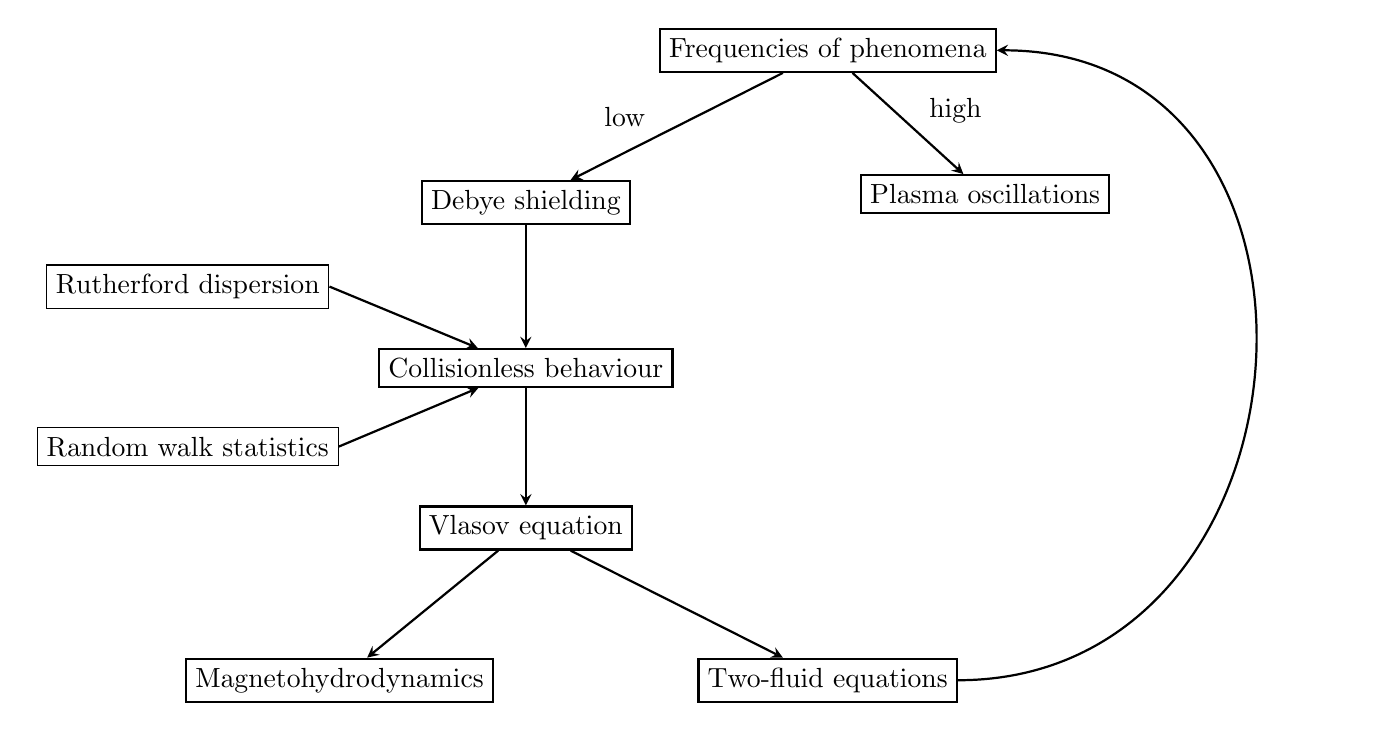
\begin{tikzpicture}[scale=1, every text node part/.style={align=center}, auto, line/.style ={draw, thick, -latex',shorten >=2pt}]
    \coordinate (freq) at (6, 4);
    \node[draw, thick] (frfr) at (freq) {Frequencies of phenomena};
    \coordinate (wifi) at (8, 2.175);
    \node[draw, thick] (hifi) at (wifi) {Plasma oscillations};
    \matrix[row sep=0.5cm,column sep=0.5cm] {
        & \node[draw, thick] (Debye) {Debye shielding}; \\
        \node[draw] (Ruth) {Rutherford dispersion}; & \\
        & \node[draw, thick] (Plas) {Collisionless behaviour}; \\
        \node[draw] (Walk) {Random walk statistics}; & \\
        & \node[draw, thick] (Vlas) {Vlasov equation}; \\
    };
    \draw[thick, -stealth] (Debye) -- (Plas);
    \draw[thick, -stealth] (Ruth.east) -- (Plas);
    \draw[thick, -stealth] (Walk.east) -- (Plas);
    \draw[thick, -stealth] (Plas) -- (Vlas);
    \coordinate (MHD) at (-0.2, -4);
    \coordinate (2F) at (6, -4);
    \node[draw, thick] (mhd) at (MHD) {Magnetohydrodynamics};
    \node[draw, thick] (2f) at (2F) {Two-fluid equations};
    \draw[thick, -stealth] (Vlas) -- (mhd);
    \draw[thick, -stealth] (Vlas) -- (2f);
    \coordinate (aux) at (7, 3.5);
    \draw[thick, -stealth] (2f.east) to[out=0, in=0, looseness=1.5] (frfr.east);
    \draw[thick, -stealth] (frfr) -- (hifi) node[pos=0.6, anchor=south west] {high};
    \draw[thick, -stealth] (frfr) -- (Debye) node[pos=0.6, anchor=south east] {low};
\end{tikzpicture}}
    \caption{Hierarchy of plasma models}
    \label{fig1-2}
\end{figure}

\section{Debye Shielding}

A careful analysis of the concept of Debye shielding, also known as \textit{Debye screening}, is essential for a deep understanding of plasma dynamics. We will consider a finite-temperature plasma composed of a very large number of electrons and ions, with equal densities initially assumed to be uniform in space. Note that these two species need not be in thermal equilibrium, as we will see later. Let $T_\text{e}$ and $T_\mathrm{i}$ be the temperatures of electrons and ions, respectively. Given that these temperatures are non-zero, the random thermal motion of the constituent particles generates tiny ephemeral fluctuations in the electrostatic potential, denoted $\phi$. Following the circular scheme of figure (\ref{fig1-2}), we admit the following assumptions:

\begin{enumerate}
    \item The plasma is assumed to be weakly collisional. In other words, we neglect higher terms in the collision approximation between constituent particles and keep only the first-order terms.
    \item We will consider species $\sigma$ as a fluid of density $n_\sigma$, temperature $T_\sigma$, and pressure $p_\sigma=n_\sigma k_\mathrm{B}T_\sigma$ moving at a mean velocity $\mathbf{u}_\sigma$. Every particle is subject to the following forces: the Lorentz force produced in part by the perturbed potential $\phi$, and the force due to fluid pressure. By taking the average over all particles, Newton's second law applied to this fluid of particles reads:
    
    \begin{equation}
        \label{eq1-1}
        m_\sigma\diff{\mathbf{u}_\sigma}{t}=q_\sigma\mathbf{E}-\frac{1}{n_\sigma}\nabla P_\sigma
    \end{equation}
    
    where $m_\sigma$ is the mass of particles of species $\sigma$, $q_\sigma$ is the particle charge, and $\mathbf{E}$ is the electric field.
\end{enumerate}

Let us assume that the observed potential perturbation obeys a time dependence sufficiently slow for the following hypotheses to be considered valid:

\begin{enumerate}
    \item The inertia term $\sim\mathrm{d}/\mathrm{d}t$ is negligible.
    \item Inductive electric fields are negligible, so $\mathbf{E}\simeq-\nabla\phi$.
    \item Any temperature gradient dissolves at a speed sufficient to ensure temperature homogeneity within each species.
    \item During the perturbation, thermal equilibrium is assumed to be maintained for each species.
\end{enumerate}

By adopting the approximations stated previously, equation (\ref{eq1-1}) is simplified into a balance between the electrostatic force and the isothermal pressure gradient:

\begin{equation}
    \label{eq1-2}
    -q_\sigma\nabla\phi-\frac{k_\mathrm{B}T_\sigma}{n_\sigma}\nabla n_\sigma\simeq0
\end{equation}

The solution to equation (\ref{eq1-2}) is trivially determined, and it allows us to establish the \textit{Boltzmann relation}:

\begin{equation}
    \label{eq1-3}
    n_\sigma(\mathbf{x},t)=n_\sigma^\square\exp\left(-\frac{q_\sigma\phi(\mathbf{x},t)}{k_\mathrm{B}T_\sigma}\right)
\end{equation}

where $n_\sigma^\square$ is a constant. It is appropriate to revisit the initial assumptions to discuss them. The relevance of the Boltzmann relation depends on the speed at which the perturbation diffuses through the plasma. If this is too fast, induced electromagnetic fields, inertia effects, and even temperature gradients can generate behaviour that deviates significantly from the Boltzmann relation. In certain situations, the Boltzmann relation remains applicable, but only to electrons, whose mass is much lower than that of ions, thus having a much larger thermal velocity, allowing the electrons to thermalise among themselves.

\vspace*{2.5pt}

\quad Let us now imagine that we introduce at position $\mathbf{x}_0$ a single test particle of charge $q_0$ into the initially unperturbed plasma, uniform on the spatial scale and neutral ($n_{\mathrm{i}}q_{\mathrm{i}}=n_{\mathrm{e}}e$). Before the introduction of the particle, the electrostatic potential was uniform due to the equality of densities $Zn_{\mathrm{i}}$ and $n_{\mathrm{e}}$. We can use this condition to set the unperturbed potential to zero. Once the particle is introduced, a perturbation will occur in the vicinity of point $\mathbf{x}_0$. Plasma particles of the same polarity as $q_0$ will be slightly repelled, while those of opposite polarity will be attracted towards $\mathbf{x}_0$. These deviations in the perturbed distribution will result in the formation of a new potential in the plasma. By virtue of the superposition principle, this new potential is equivalent to the simple superposition of the potential created by the introduced charge $q_0$ and that created by the displaced plasma particles. The slight displacement of plasma particles is designated by the terms \textit{shielding}, \textit{masking}, or \textit{screening} of the introduced charge, as it depletes the long-range influence of the introduced particle. The perturbation of the distribution of the plasma's constituent particles around the introduced charge is called a \textit{shielding cloud}. It should be emphasized that the polarity of the shielding cloud is opposite to that of $q_0$. The potential generated by Debye shielding is described by Poisson's equation, whose potential sources are the particle of charge $q_0$ and its associated shielding cloud:

\begin{equation*}
    \nabla^2\phi(\mathbf{x})=-\frac{1}{\varepsilon_0}\left(q_0\delta^3(\mathbf{x}-\mathbf{x}_0)+\sum_{\sigma}n_\sigma(\mathbf{x})q_\sigma\right)
\end{equation*}

Provided that the particle is introduced into the plasma with sufficient delicacy, the plasma's response will be determined by the Boltzmann relation (\ref{eq1-3}). The perturbation is consequently assumed infinitesimal; we take advantage of this by establishing the following approximation:

\begin{equation}
    |q_\sigma\phi(\mathbf{x})|\ll k_\mathrm{B}T_\sigma\implies n_\sigma(\mathbf{x})\simeq n_\sigma^\square\left(1-\frac{q_\sigma\phi(\mathbf{x})}{k_\mathrm{B}T_\sigma}\right)
\end{equation}

\begin{equation}
    \label{eq1-6}
    \nabla^2\phi(\mathbf{x})=-\frac{1}{\varepsilon_0}\left(q_0\delta^3(\mathbf{x}-\mathbf{x}_0)+\sum_{\sigma}\left(1-\frac{q_\sigma\phi(\mathbf{x})}{k_\mathrm{B}T_\sigma}\right)n_\sigma^\square q_\sigma\right)
\end{equation}

We can simplify (\ref{eq1-6}) by the assumption of neutrality:

\begin{equation}
    \label{eq1-7}
    \sum_\sigma n_\sigma^\square q_\sigma=0\implies\nabla^2\phi(\mathbf{x})=-\frac{1}{\varepsilon_0}\left(q_0\delta^3(\mathbf{x}-\mathbf{x}_0)-\sum_\sigma\frac{n_\sigma^\square q_\sigma^2}{k_\mathrm{B}T_\sigma}\phi(\mathbf{x})\right)
\end{equation}

We define the Debye length of species $\sigma$ and the effective Debye length as follows:

\begin{equation}
    \label{eq1-9}
    \lambda_\sigma^2=\frac{\varepsilon_0k_\mathrm{B}T_\sigma}{n_\sigma^\square q_\sigma^2}\implies\frac{1}{\lambda_\mathrm{D}^2}=\sum_\sigma\frac{1}{\lambda^2_\sigma}\quad\implies  \quad\nabla^2\phi(\mathbf{x})-\frac{1}{\lambda_\mathrm{D}^2}\phi=-\frac{q_0}{\varepsilon_0}\delta^3(\mathbf{x}-\mathbf{x}_0)
\end{equation}

It is possible to solve (\ref{eq1-9}) by applying Gauss's law; however, a more general approach is to use the Fourier transform, and we do so to illustrate a more formal and powerful mathematical technique. The first step consists of defining the Fourier transform in three dimensions:

\begin{equation*}
    \Tilde{\phi}(\mathbf{k})=\iiint_{\mathbb{R}^3}\phi(\mathbf{x})e^{-i\mathbf{k}\cdot\mathbf{x}}\,\mathrm{d}^3\mathbf{x}\implies\phi(\mathbf{x})=\frac{1}{(2\pi)^3}\iiint_{\mathbb{R}^3}\Tilde{\phi}(\mathbf{k})e^{i\mathbf{k}\cdot\mathbf{x}}\,\mathrm{d}^3\mathbf{k}
\end{equation*}

The transform of the Dirac distribution is simply given as follows:

\begin{gather*}
    \iiint_{\mathbb{R}^3}\delta^3(\mathbf{x}-\mathbf{x}_0)e^{-i\mathbf{k}\cdot\mathbf{x}}\,\mathrm{d}^3\mathbf{x}=e^{-i\mathbf{k}\cdot\mathbf{x}_0}\implies \delta^3(\mathbf{x}-\mathbf{x}_0)=\frac{1}{(2\pi)^3}\iiint_{\mathbb{R}^3}e^{i\mathbf{k}\cdot(\mathbf{x}-\mathbf{x}_0)}\,\mathrm{d}^3\mathbf{k}\\
    \iiint_{\mathbb{R}^3}\nabla^2\phi(\mathbf{x})e^{-i\mathbf{k}\cdot\mathbf{x}}\,\mathrm{d}^3\mathbf{x}=(i\mathbf{k})^2\iiint_{\mathbb{R}^3}\phi(\mathbf{x}) e^{-i\mathbf{k}\cdot\mathbf{x}}\,\mathrm{d}^3\mathbf{k}
\end{gather*}

\begin{equation*}
    -\left(\mathbf{k}^2+\frac{1}{\lambda_\mathrm{D}^2}\right)\Tilde{\phi}(\mathbf{k})=-\frac{q_0}{\varepsilon_0}e^{-i\mathbf{k}\cdot\mathbf{x_0}}\implies\Tilde{\phi}(\mathbf{k})=\frac{q_0/\varepsilon_0}{\mathbf{k}^2+\lambda_\mathrm{D}^{-2}}e^{-i\mathbf{k}\cdot\mathbf{x_0}}
\end{equation*}

Let $\mathbf{k}\cdot\left(\mathbf{x}-\mathbf{x}_0\right)=k \left\|\mathbf{x}-\mathbf{x}_0\right\|\cos(\vartheta)$; we evaluate the integral using a spherical coordinate system:

\begin{align*}
    \phi(\mathbf{x})&=\frac{1}{(2\pi)^3}\int_{0}^{2\pi}\int_{0}^{\pi}\int_{0}^{\infty}\frac{q_0/\varepsilon_0}{k^2+\lambda_\mathrm{D}^{-2}}e^{ik \left\|\mathbf{x}-\mathbf{x}_0\right\|\cos{\left(\vartheta\right)}}k^2\sin(\vartheta)\,\mathrm{d}k\,\mathrm{d}\vartheta\,\mathrm{d}\varphi=\\
    &=\frac{q_0}{(2\pi)^3\varepsilon_0}\int_{0}^{2\pi}\mathrm{d}\varphi\int_0^{\infty}\frac{k^2}{k^2+\lambda_\mathrm{D}^{-2}}\int_{0}^{\pi}\left(-\frac{\left(-ik \left\|\mathbf{x}-\mathbf{x}_0\right\|\sin(\vartheta)\right)}{ik \left\|\mathbf{x}-\mathbf{x}_0\right\|}\right)e^{ik \left\|\mathbf{x}-\mathbf{x}_0\right\|\cos{\left(\vartheta\right)}}\,\mathrm{d}\vartheta\,\mathrm{d}k=\\
    &=\frac{iq_0}{4\pi^2 \varepsilon_0 \left\|\mathbf{x}-\mathbf{x}_0\right\|}\int_0^\infty \frac{k}{k^2+\lambda_{\mathrm{D}}^{-2}}\left[e^{ik \left\|\mathbf{x}-\mathbf{x}_0\right\|\cos{\left(\vartheta\right)}}\right]\biggr|_{0}^{\pi}\,\mathrm{d}k=\\
    &=\frac{i q_0}{4\pi \varepsilon_0 \left\|\mathbf{x}-\mathbf{x}_0\right\|}\left(\int_0^\infty \frac{ke^{-ik \left\|\mathbf{x}-\mathbf{x}_0\right\|}}{k^2+\lambda_{\mathrm{D}}^{-2}}\,\mathrm{d}k+\int_0^\infty\frac{-ke^{ik \left\|\mathbf{x}-\mathbf{x}_0\right\|}}{k^2+\lambda_{\mathrm{D}}^{-2}}\,\mathrm{d}k\right)=\big\{k\to-k\big\}=\\
    &=\frac{iq_0}{4\pi \varepsilon_0 \left\|\mathbf{x}-\mathbf{x}_0\right\|}\int_{-\infty}^\infty \frac{ke^{-ik\|\mathbf{x}-\mathbf{x_0}\|}}{k^2+\lambda_{\mathrm{D}}^{-2}}\,\mathrm{d}k
\end{align*}

To evaluate the last integral, we shall resort to complex analysis. The integrand has two poles, $k=i\lambda_\mathrm{D}^{-1}$ and $k=-i\lambda_\mathrm{D}^{-1}$. Notice that the integrand vanishes when $|k|\to\infty$ and $\Im{k}\leq 0$; this motivates us to construct a semi-circular loop of radius $R$ in the lower complex semi-plane, and then use Jordan's lemma to eliminate the integral over the arc when taking the limit as $R\to\infty$. Formally, we define $[-R,R]\cup\Gamma=[-R,R]\cup\left\{z\in \mathbb{C}:|z|=R,\, \Im{z}<0\right\}$ as our integration path traversed clockwise. Consider the integral over the arc, where $z=Re^{i\theta}$ with $\theta\in(\pi,2\pi)$ and $R>\lambda_{\mathrm{D}}^{-1}$:

\begin{align*}
    \left|\int_\Gamma\frac{ze^{-iz\|\mathbf{x}-\mathbf{x_0}\|}}{z^2+\lambda_{\mathrm{D}}^{-2}}\,\mathrm{d}z\right|&\leq\int_\pi^{2\pi}\frac{R^2e^{R \sin{\left(\theta\right)}\|\mathbf{x}-\mathbf{x_0}\|}}{\left|R^2e^{2i\theta}+\lambda_{\mathrm{D}}^{-2}\right|}\,\mathrm{d}\theta\leq\int_0^\pi \frac{R^2e^{-R \sin{\left(\theta\right)} \left\|\mathbf{x}-\mathbf{x}_0\right\|}}{R^2-\lambda_{\mathrm{D}}^{-2}}\,\mathrm{d}\theta=\\
    &=\frac{2R^2}{R^2-\lambda_{\mathrm{D}}^{-2}}\int_0^{\pi/2}{e^{-R \sin{\left(\theta\right)}}\left\|\mathbf{x}-\mathbf{x}_0\right\|}\,\mathrm{d}\theta\leq\bigg\{\sin{\theta}\geq\frac{2}{\pi}\theta,\theta\in \left[0,\frac{\pi}{2}\right]\bigg\}\leq\\
    &\leq \frac{2R^2}{R^2-\lambda_{\mathrm{D}}^{-2}}\int_0^{\pi/2}e^{-\frac{2}{\pi}R\theta \left\|\mathbf{x}-\mathbf{x}_0\right\|}\,\mathrm{d}\theta=-\frac{\pi R}{R^2-\lambda_{\mathrm{D}}^{-2}}\frac{1}{\left\|\mathbf{x}-\mathbf{x}_0\right\|}\left[e^{-\frac{2}{\pi}R\theta \left\|\mathbf{x}-\mathbf{x}_0\right\|}\right]_0^{\pi/2}=\\
    &=\frac{\pi R}{R^2-\lambda_{\mathrm{D}}^{-2}}\frac{1}{\left\|\mathbf{x}-\mathbf{x}_0\right\|}\left(1-e^{-R \left\|\mathbf{x}-\mathbf{x}_0\right\|}\right)\longrightarrow 0\quad \left(R\to\infty\right)
\end{align*}

while the integral over $[-R,R]$ converges to the sought-after integral as $R\to\infty$ by construction. Since we have chosen the clockwise orientation, we have to artificially add a negative sign to the residue evaluation:

\begin{equation*}
    \int_{-\infty}^\infty \frac{ke^{-ik \left\|\mathbf{x}-\mathbf{x}_0\right\|}}{k^2+\lambda_{\mathrm{D}}^{-2}}\,\mathrm{d}k=-2\pi i\lim_{k\to -i\lambda_{\mathrm{D}}^{-1}}\left(k+i\lambda_{\mathrm{D}}^{-1}\right)\frac{ke^{-ik \left\|\mathbf{x}-\mathbf{x}_0\right\|}}{k^2+\lambda_{\mathrm{D}}^{-2}}=\frac{\pi}{i}\exp{\left(-\frac{\left\|\mathbf{x}-\mathbf{x}_0\right\|}{\lambda_{\mathrm{D}}}\right)}
\end{equation*}

The form of the solution is commonly known by the term \textit{Yukawa potential}:

\begin{equation}
    \label{yukawa}
    \phi(\mathbf{x})=\frac{q_0}{4\pi \varepsilon_0}\frac{1}{\left\|\mathbf{x}-\mathbf{x}_0\right\|}\exp{\left(-\frac{\left\|\mathbf{x}-\mathbf{x}_0\right\|}{\lambda_D}\right)}
\end{equation}

It is now appropriate to examine the obtained solution. In the immediate vicinity of the particle of charge $q_0$, when the inequality $\|\mathbf{x}-\mathbf{x}_0\|\ll\lambda_\mathrm{D}$ is well verified, the potential is equivalent to that which this particle exerts in a vacuum. As one moves farther from the introduced particle, the potential vanishes due to screening by the shielding cloud. The validity of Debye screening holds only when the total plasma particle density is sufficiently high, that is, when $N_{\mathrm{D}}=n\lambda_\mathrm{D}^3\gg1$. It will be shown later that this condition precisely corresponds to the hypothesis of a weakly collisional plasma, one of the initial approximations in this section. Furthermore, the concept of Debye shielding is only relevant if the Debye length is considerably smaller than the spatial dimensions of the plasma. Otherwise, any plasma particle is necessarily inside the shielding cloud. It should be noted that the introduced particle could be any particle of the plasma. However, from a statistical point of view, such a particle, selected at random, moves at a defined velocity and is no longer characterized by the thermal speed of its species.

\section{Quasi-neutrality}

The study of Debye shielding relies on the hypothesis that the plasma was initially neutral, i.e., that electron and ion densities were equal and uniform at the initial instant. In this section, we demonstrate that the hypothesis we have formulated is excellent. More precisely, the result established in this section is that the plasma exhibits, remarkably, a state of neutrality when the Debye length is microscopic compared to the dimensions of the plasma. Indeed, conventional plasmas manifest a propensity to be quasi-neutral, because they generally do not possess sufficient internal energy to reach a non-neutral state over distances that considerably exceed the Debye length.  We will demonstrate the argument by considering a plasma initially in a state of neutrality, with electrons at temperature $T_\text{e}$. Consider a sphere susceptible to spontaneously depleting all its electrons due to thermal fluctuations. We evaluate the maximum radius of such a sphere and denote it $R_\text{max}$. The depletion of electrons causes them to stop at the surface of the sphere. The energy required to create a space devoid of electrons is indeed the energy of the electrostatic field created by the ions remaining inside the sphere. Gauss's law allows us to determine the form of the electrostatic field under consideration, and consequently, the potential energy of the configuration:

\begin{equation*}
    \nabla\cdot\mathbf{E}\equiv\frac{1}{r^2}\frac{\partial}{\partial r}\left(r^2E_r\right)=\frac{\rho}{\varepsilon_0}=\frac{n_ee}{\varepsilon_0}
\end{equation*}

where we have omitted the azimuthal and polar terms due to the symmetry. The solution follows trivially:

\begin{equation*}
    \mathbf{E}(\mathbf{r})=\frac{n_ee}{3\varepsilon_0}\mathbf{r}
\end{equation*}

\begin{equation*}
    W=\frac{\varepsilon_0}{2}\iiint_{B(\mathbf{0},R)}\mathbf{E}^2\,\mathrm{d}^3\mathbf{r}=2\pi\varepsilon_0\times\frac{e^2n_e^2}{9\varepsilon_0^2}\int_0^{R_\text{max}}r^4\,\mathrm{d}r=\frac{2\pi e^2n_e^2}{45\varepsilon_0} R_\text{max}^5
\end{equation*}

The potential energy is equal to the net initial kinetic energy of all evacuated electrons, hence:

\begin{equation*}
    K=\frac{3}{2}n_ek_\mathrm{B}T\times\frac{4}{3}\pi R_{\text{max}}^3 = 2\pi k_\mathrm{B}Tn_eR_\text{max}^3
\end{equation*}

\begin{equation*}
    R_\text{max}^2=45\frac{\varepsilon_0k_\mathrm{B}T}{e^2n_e}=45\lambda_e^2
\end{equation*}

The estimation $R_\text{max}\lesssim7\lambda_e$ follows. The maximum radius of a space completely devoid of electrons is, for its part, limited to a few Debye lengths. Considering the extremely low probability that the velocities of all these electrons are directed radially relative to a common centre, we deduce that plasmas are indeed quasi-neutral on a scale that largely exceeds their Debye length. It emerges from this analysis that the extent of the non-neutral region caused by a potential perturbation, i.e. of the shielding cloud, does not exceed the order of the associated Debye length.

\section{Collisions in plasmas: first considerations}

Now, we study a simple collision between two plasma particles interacting only by the electrostatic force. Let there be two particles of possibly different species $\sigma$ and $\rho$, masses $m_\sigma$ and $m_\rho$, charges $q_\sigma$ and $q_\rho$, and let $\mathbf{r}_\sigma$ and $\mathbf{r}_\rho$ denote their respective positions. For the sake of relevance, we will neglect the magnetic fields produced by the motion of the two charges, as well as the effect of electromagnetic radiation; indeed, for small charges moving with non-relativstic velocities, present as such in plasmas, the interaction of a charge with the magnetic field of the other is completely negligible, so we can consider only the electrostatic interaction. The radiation associated with the total EM field due to the acceleration of both charges is well-known to be orders of magnitude weaker than typical electrostatic interactions, so we can consider the system's total energy as conserved without any issue.

\vspace*{2.5pt}

\quad Starting from Newton's law, the time evolution equations for the positions $\mathbf{r}_\sigma$ and $\mathbf{r}_\rho$ read:

\begin{equation*}
    m_\sigma\frac{\mathrm{d}^2\mathbf{r}_\sigma}{\mathrm{d}t^2}=\frac{q_\sigma q_\rho}{4\pi\varepsilon_0}\frac{\mathbf{r}_\sigma-\mathbf{r}_\rho}{\|\mathbf{r}_\sigma-\mathbf{r}_\rho\|^3}\quad\quad\quad m_\rho\frac{\mathrm{d}^2\mathbf{r}_\rho}{\mathrm{d}t^2}=\frac{q_\sigma q_\rho}{4\pi\varepsilon_0}\frac{\mathbf{r}_\rho-\mathbf{r}_\sigma}{\|\mathbf{r}_\rho-\mathbf{r}_\sigma\|}
\end{equation*}

Let $\mathbf{u}_\sigma$ be the velocity of the first particle in the frame of the other, when the two particles are infinitely far from each other. It is useful to introduce the substitution defined by the centre-of-mass and the relative position of the incident particle with respect to the target particle, $\mathbf{R}_{\mathrm{CM}}$ and $\mathbf{r}$: 

\begin{gather*}
    \mathbf{r}=\mathbf{r}_\sigma-\mathbf{r}_\rho,\quad \mathbf{R}_{\mathrm{CM}}=\frac{m_\sigma \mathbf{v}_\sigma+m_\rho \mathbf{v}_\rho}{m_\sigma+m_\rho}\,\implies\,\mathbf{r}_\sigma=\mathbf{R}_{\mathrm{CM}}+\frac{m_\rho}{m_\sigma+ m_\rho}\mathbf{r},\quad \mathbf{r}_\rho=\mathbf{R}_{\mathrm{CM}}-\frac{m_\sigma}{m_\sigma+m_\rho}\mathbf{r}\\
    \frac{\mathrm{d}\mathbf{r}}{\mathrm{d}t}=\mathbf{v}_{\sigma\to\rho}(t)\quad\text{and}\quad \frac{\mathrm{d}\mathbf{R}_\sigma}{\mathrm{d}t}=\mathbf{v}_{\mathrm{CM}}=\text{const.}\\
    \frac{\mathrm{d}^2\mathbf{r}}{\mathrm{d}t^2}=\left(\frac{1}{m_\sigma}+\frac{1}{m_\rho}\right)\frac{q_\sigma q_\rho}{4\pi\varepsilon_0}\frac{\mathbf{r}}{\|\mathbf{r}\|^3}\quad\text{and}\quad \frac{\mathrm{d}^2 \mathbf{R}_{\mathrm{CM}}}{\mathrm{d}t^2}=\mathbf{0}
\end{gather*}

where we conveniently define the reduced mass $\mu_{\sigma\rho}=m_\sigma m_\rho/\left(m_\sigma+m_\rho\right)$. The dynamics of the first particle is thus identical to that of a particle of mass $\mu_{\sigma\rho}$ and charge $q_\sigma$ around a fixed charge $q_\rho$, as illustrated in (\ref{fig1-3}). Let us define the axis $\mathbf{\hat{z}}=\mathbf{v}_{\sigma\to\rho}/\|\mathbf{v}_{\sigma\to\rho}\|$ and the axes $\mathbf{\hat{x}}$ and $\mathbf{\hat{y}}=\mathbf{\hat{z}}\times\mathbf{\hat{x}}$ as in Figure (\ref{fig1-3}): 

\begin{figure}[H]
    \centering
    \begin{tikzpicture}[scale=1, every text node part/.style={align=center}, auto, line/.style ={draw, thick, -latex',shorten >=2pt}]
    \draw[thick] plot[variable=\t, samples=1000, domain=-5.5:4.75] ({\t-0.4}, {1.5+0.40124073018*\t+sqrt(0.142612664+0.16269649092*\t*\t)});
    \coordinate (O) at (0, 0);
    \coordinate (init) at (-5, 1.55);
    \coordinate (fin) at (3.3, 4.53);
    \coordinate (t) at (-0.4, 1.87);
    \node[anchor=north west] (q2) at (O) {$q_2$};
    \draw[black, fill] (O) circle [radius=2pt];
    \node[anchor=south west] (q1init) at (init) {$\mu, q_1$};
    \draw[black, fill] (init) circle [radius=2pt];
    \node[anchor=south east] (q1t) at (t) {$\mu, q_1$};
    \draw[black, fill] (t) circle [radius=2pt];
    \node[anchor=south east] (q1fin) at (fin) {$\mu, q_1$};
    \draw[black, fill] (fin) circle [radius=2pt];
    \coordinate (-z) at (-6.5, 0);
    \coordinate (+z) at (4.25, 0);
    \draw[-stealth, thick] (-z) -- (+z);
    \node[anchor=south east] (z) at (+z) {$\mathbf{\hat{z}}$};
    \coordinate (-x) at (0, -0.5);
    \coordinate (+x) at (0, 6);
    \draw[-stealth, thick] (-x) -- (+x);
    \node[anchor=north east] (x) at (+x) {$\mathbf{\hat{x}}$};
    \draw[thick, -Stealth] (O) -- (t) node[pos=0.45, anchor=east] {$\mathbf{r}$};
    \draw[thick, dashed] (-6.15, 1.5) -- (4.20, 1.5);
    \draw[stealth-stealth, thick] (-4, 0) -- (-4, 1.5) node[midway, anchor=west] {$b$};
    \draw[-Stealth, thick, line width=1.25pt] (init) -- (-3.5, 1.56) node[pos=0.75, anchor=south west] {$\mathbf{v}\simeq\mathbf{v}_1$};
    \draw[-Stealth, thick, line width=1.25pt] (t) -- (1, 2.5) node[pos=0.93, anchor=north west] {$\mathbf{v}$};
    \draw[-Stealth, thick, line width=1.25pt] (fin) -- (4.45, 5.45) node[pos=0.6, anchor=north west] {$\mathbf{v}\simeq\mathbf{v}_\infty$};
    \draw[thick, dashed] plot[variable=\t, samples=1000, domain=-0.75:4.5] ({\t}, {0.78*\t});
    \draw[thick, dashed] plot[variable=\t, samples=1000, domain=-1.75:4.5] ({\t}, {0.78*\t+1.85});
    \draw[thick, stealth-stealth] (2.8, {0.78*2.8+1.85}) -- (3.697164884, {0.78*3.697164884}) node[midway, anchor=south west] {$b$};
    \draw[thick, -stealth] ({1.923076913+1.5}, 1.5) arc (0:37.954:1.5);
    \node[thick] at (3, 1.84) {$\theta_c$};
\end{tikzpicture}
    \caption{Illustration of the binary Coulomb collision problem.}
    \label{fig1-3}
\end{figure}

The system can be solved by a brute-force method; on the contrary, we shall exploit the fact that the electrostatic force from the fixed charge is a central force, and as such the Laplace-Runge-Lenz vector associated with the incident particle's orbit is conserved. Notice that the incident particle's angular momentum about the fixed charge is also a conserved quantity; this allows us to express the Laplace-Runge-Lenz vector in terms of incident and exiting velocities and angles:

\begin{equation}
    \label{eq-1-29}
    \boldsymbol{\epsilon}_\sigma=-\frac{4\pi\varepsilon_0\mathbf{p}_\sigma\times\mathbf{\mathcal{L}}_\sigma}{\mu_{\sigma\rho}q_\sigma q_\rho}-\mathbf{\hat{r}}=
    -\frac{4\pi\varepsilon_0\mu_{\sigma\rho}v_{\sigma\to\rho}\,\mathbf{\hat{z}}}{\mu_{\sigma\rho}q_\sigma q_\rho}\times\left(-\mu_{\sigma\rho}v_{\sigma\to\rho} b\,\mathbf{\hat{y}}\right)-\left(-\mathbf{\hat{z}}\right)=-\frac{4\pi\varepsilon_0\mu_{\sigma\rho}v_{\sigma\to\rho}^2b}{q_\sigma q_\rho}\,\mathbf{\hat{x}}+\mathbf{\hat{z}}
\end{equation}

The exiting velocity is equal to the incident velocity in norm by hypothesis of conservation of energy:

\begin{equation*}
    \boldsymbol{\epsilon}_\sigma=-\frac{4\pi\varepsilon_0}{\mu_{\sigma\rho}q_\sigma q_\rho}\left[\mu_{\sigma\rho}\left(v_{\sigma\to\rho}\cos(\theta_c)\,\mathbf{\hat{z}}+v_{\sigma\to\rho}\sin(\theta_c)\,\mathbf{\hat{x}}\right)\right]\times\left(-\mu_{\sigma\rho}v_{\sigma\to\rho} b\,\mathbf{\hat{y}}\right)-\left[\cos(\theta_c)\,\mathbf{\hat{z}}+\sin(\theta_c)\,\mathbf{\hat{x}}\right]=
\end{equation*}

\begin{equation}
    \label{eq-1-31}
    =\left[\sin(\theta_c)-\frac{4\pi\varepsilon_0\mu_{\sigma\rho}v_{\sigma\to\rho}^2b}{q_\sigma q_\rho}\cos(\theta_c)\right]\mathbf{\hat{x}}+\left[\frac{4\pi\varepsilon_0\mu_{\sigma\rho}v_{\sigma\to\rho}^2b}{q_\sigma q_\rho}\sin(\theta_c)-\cos(\theta_c)\right]\mathbf{\hat{z}}
\end{equation}

By comparing (\ref{eq-1-29}) and (\ref{eq-1-31}), in particular the components along $\mathbf{\hat{z}}$, we can establish the expression for the deflection angle in the target particle's frame, $\theta_c$:

\begin{equation}
    \label{eq-1-32}
    \sin(\theta_c)=\frac{q_\sigma q_\rho}{4\pi\varepsilon_0\mu_{\sigma\rho}v_{\sigma\to\rho}^2b}\left[1+\cos(\theta_c)\right]\Longleftrightarrow\tan\left(\frac{\theta_c}{2}\right)=\frac{q_\sigma q_\rho}{4\pi\varepsilon_0\mu_{\sigma\rho}v_{\sigma\to\rho}^2b}
\end{equation}

Let us define by $b_{\pi/2}$ the impact parameter corresponding to a deflection of $\theta_c=\pi/2$, then:

\begin{equation}
    b_{\pi/2}=\frac{q_\sigma q_\rho}{4\pi\varepsilon_0\mu_{\sigma\rho}v_{\sigma\to\rho}^2}
\end{equation}

The deflection angle in the laboratory frame is different, however. We can write the outgoing velocities in both the laboratory and the target particle's frame as follows:

\begin{equation*}
    \mathbf{v'}\bigr|_\text{lab}=\diff{\mathbf{R}_\text{CM}}{t}+\frac{m_\rho}{m_\sigma+m_\rho}\diff{\mathbf{r}}{t}=\left[v_\text{CM}+\frac{m_\rho v_{\sigma\to\rho}}{m_\sigma+m_\rho}\cos(\theta_c)\right]\mathbf{\hat{z}}+\frac{m_\rho v_{\sigma\to\rho}}{m_\sigma+m_\rho}\sin(\theta_c)\,\mathbf{\hat{x}}
\end{equation*}

from which we can determine exactly the deflection angle $\chi_c$ in the laboratory frame:

\begin{equation*}
    \cot(\chi_c)=\frac{v_\text{CM}+\frac{m_\rho v_{\sigma\to\rho}}{m_\sigma+m_\rho}\cos(\theta_c)}{\frac{m_\rho v_{\sigma\to\rho}}{m_\sigma+m_\rho}\sin(\theta_c)}=\frac{v_\text{CM}}{v_{\sigma\to\rho}}\frac{m_\sigma+m_\rho}{m_\rho}\csc(\theta_c)+\cot(\theta_c)
\end{equation*}

\begin{equation}
    v_\text{CM}=\frac{m_\sigma v_{\sigma\to\rho}}{m_\sigma+m_\rho}\implies\cot(\chi_c)=\frac{m_\sigma}{m_\rho}\csc(\theta_c)+\cot(\theta_c)
\end{equation}

We shall now postpone our considerations on collisions in order to first give a clear objective of the goal we're seeking to achieve: determining the collision frequencies between species and concluding that plasmas are indeed weakly collisional. 

\subsection{Digression: cross-sections}

The cross-section associated with a particular collisional phenomenon determines the probability that the considered phenomenon occurs; more precisely, a cross-section is represented by a surface area associated with each incident particle taking part in the collisional phenomenon.

\vspace*{2.5pt}

\quad Consider two species of particles, $\sigma$ and $\rho$, each associated with its particle distribution function, $f_\sigma(\mathbf{x},\mathbf{v},t)$ and $f_\rho(\mathbf{x},\mathbf{v},t)$. We shall arbitrarily refer to the first species as incident and the latter as target species. Let us now focus on the group of target particles travelling at velocities (by abuse of notation) in the range $\mathbf{v}_\rho+\mathrm{d^3}\mathbf{v}_\rho$, and whose number density is therefore $f_\rho(\mathbf{x},\mathbf{v}_\rho,t)\,\mathrm{d^3}\mathbf{v}_\rho$ within some volume $\mathrm{d^3}\mathbf{x}$. Now, for each particle of the group of incident particles travelling at velocities $\mathbf{v}_\sigma + \mathrm{d^3}\mathbf{v}_\sigma$, the target group offers a total collisional cross section quantified by $f_\rho(\mathbf{x},\mathbf{v}_\rho,t)\sigma_{\sigma\to\rho}(\mathbf{v}_\sigma,\mathbf{v}_\rho)\,\mathrm{d^3}\mathbf{v}_\rho$. We now move into the reference frame of the target group, so that within a time $\mathrm{d}t$, the incident group sweeps out a path of length $\left\|\mathbf{v}_\sigma -\mathbf{v}_\rho\right\|\,\mathrm{d}t$ within the same volume $\mathrm{d^3}\mathbf{x}$. The probability that a single incident particle undergoes a collision within thetime $\mathrm{d}t$ is expressed as:

\begin{equation}
    \label{eq-preliminaries-13}
    P(\text{collision}|\mathbf{v}_\sigma,\mathbf{v}_\rho)\,\mathrm{d^3}\mathbf{v}_\rho\,\mathrm{d}t=f_\rho(\mathbf{x},\mathbf{v}_\rho,t)\sigma_{\sigma\to\rho}(\mathbf{v}_\sigma,\mathbf{v}_\rho)\left\|\mathbf{v}_\sigma-\mathbf{v}_\rho\right\|\,\mathrm{d^3}\mathbf{v}_\rho\,\mathrm{d}t
\end{equation}

In fact, the proper definition of a collisional cross-section is specifically via this last expression. Therefore, we see that the cross-section is dependent on the target particle distribution function and the relative velocity between the incident and the target groups, and it usually depends only on the norm of the relative velocity. In fact, (\ref{eq-preliminaries-13}) can be thought of as an integral kernel for evaluating averages of quantities that depend on collisions, i.e. evaluating average collision number frequency, average momentum and energy dissipation or diffusion frequencies, etc. We shall now illustrate the first example, that is the total collision number frequency. We can express the total number of collisions $\mathrm{d}N$ within time $\mathrm{d}t$ and volume $\mathrm{d^3}\mathbf{x}$ (thus $N$ is the collision number \textit{density}) simply as the product of the incident group density and the probability of a collision, and simply integrate over all admissible incident and target groups:

\begin{equation}
    \label{eq-preliminaries-14}
    \nu_{\mathrm{collision}}(\mathbf{x},t)=\frac{\mathrm{d}N}{\mathrm{d}t}=\iiint_{\mathbb{R}^3}\iiint_{\mathbb{R}^3}f_\sigma(\mathbf{x},\mathbf{v}_\sigma,t)f_\rho(\mathbf{x},\mathbf{v}_\rho,t)\sigma_{\sigma\to\rho}(\mathbf{v}_\sigma,\mathbf{v}_\rho)\left\|\mathbf{v}_\sigma-\mathbf{v}_\rho\right\|\,\mathrm{d^3}\mathbf{v}_\rho\,\mathrm{d^3}\mathbf{v}_\sigma
\end{equation}

which marks the end of this digression.

\vspace*{2.5pt}

\quad Returning to the problem of Coulomb collisions, let us now consider a quasi-neutral plasma that is not undergoing fusion, i.e. in which the conservation of particle number is exact. We would now like to use the conservation of particle number to determine the cross-section associated with a single binary Coulomb collision, and apply the result to (\ref{eq-preliminaries-14}). This is unfortunately not a straightforward task because the interaction between plasma particles is not given by the simple Coulomb electrostatic interaction, i.e. the electrostatic force in a plasma is not governed by an inverse-square law, but has an additional decaying factor as given by (\ref{yukawa}), i.e. due to the shielding cloud. Notably, the Yukawa potential does not present any useful symmetries, and as such we cannot associate a Laplace-Runge-Lenz vector-like conserved quantity to the incident particle's orbit. Nonetheless, it is still worth considering the collisional cross-section of a simple Coulomb potential; due to the decay factor, we only expect to effectively \textit{overestimate} the true cross-sections, and by extension the true collisional frequencies in plasmas. We shall later conclude for the Yukawa cross-section.

\vspace*{2.5pt}

\quad We shall therefore make the following assumption and argue why it is worth considering. For each incident particle entering into Coulomb collisions with a group of target particles such that, in the reference frame of the latter, the incident particle moves at velocity $\mathbf{v}_{\sigma\to\rho}$, we assume that its dynamics is sufficiently approximated by a sequence of deflections with some angle $\theta_c$, i.e. that we can treat each encounter with a target particle separately and sequentially. This is true to the realistic situation for small angles of deflection, since such trajectories experience little deflection  in the \textit{long-range} interaction, i.e. on length scales greater than the impact parameter; however, a seeming contradiction is that plasmas are defined by the great number of particles within a Debye sphere. This would imply that any incident particle interacts almost simultaneously with a very large number of target particles. On the contrary, one may convince oneself that, by averaging over target particle groups, we would somehow recover the true dynamics due to the Yukawa potential field. In fact, the converse is true; the Yukawa potential, due to its weak long-range interaction, enables us to consider only those interactions whose impact parameter is within the scale of the Debye length. The large number of particles in a Debye sphere allow us to consider a statistically most probable situation where the majority of collisions are weakly-deflecting, and amount to small, globally uncorrelated random-walk-like steps in the phase space; indeed, a simultaneous superposition of independent interactions is indistinguishable from a sequence of independent binary interactions, i.e. from a Markov process. Our procédé is to therefore consider those Coulomb collisions with impact parameters within the scale of the Debye length and, at the same time, the weakly-deflecting ones; effectively, we restrain the domain of the impact parameter to $b\in[b_{\pi/2},\lambda_{\mathrm{D}}]$. We will retouch this subject later when considering the Balescu-Lenard operator in the chapter on the theory of transport.

\vspace*{2.5pt}

\quad In virtue of conservation of particle number, we consider an annular surface area $2\pi b\,\mathrm{d}b$ through which incident particles propagate with a velocity $\mathbf{v}_{\sigma\to\rho}$ with respect to a single target particle, hence undergoing an angular deflection between $\theta_c$ and $\theta_c+\mathrm{d}\theta_c$. The deflected particles then pierce the solid angle $\mathrm{d}\Omega=2\pi\sin(\theta_c)\mathrm{d}\theta_c$; the following relation is established:

\begin{equation}
    \frac{\mathrm{d}\sigma(\theta_c)}{\mathrm{d}\Omega}\,\mathrm{d}\Omega=2\pi b\,\mathrm{d}b\implies\frac{\mathrm{d}\sigma(\theta_c)}{\mathrm{d}\Omega}=\frac{b}{\sin(\theta_c)}\left|\frac{\mathrm{d}b}{\mathrm{d}\theta_c}\right|
\end{equation}

The sought derivative is found via eq. (\ref{eq-1-32}), giving the \textit{Rutherford cross-section} relation:

\begin{equation}
    \frac{\mathrm{d}\sigma}{\mathrm{d}\Omega}(\theta_c)=\frac{1}{4}\left(\frac{q_1q_2}{4\pi\varepsilon_0\mu v_0^2}\csc^2\left(\frac{\theta_c}{2}\right)\right)^2=\frac{1}{4}\left(\frac{b_{\pi/2}}{\sin^2(\theta_c/2)}\right)^2
\end{equation}

\subsection{Collisions with small and large angles of deflection}

We now examine the validity of the approximation that plasmas are weakly collisional, i.e., that collisions resulting in small deflections, whose cumulative effect is equivalent to a collision resulting in a large deflection, are vastly more frequent than those resulting in a large deflection. Let us exemplarily analyse the collisional momentum dissipation; specifically, we consider two plasma species moving frontally at different mean velocities. Say $\sigma$ is the incident particle species, and $\rho$ the target particle species. Transferring into the reference frame of the target particle species, we expect the incident particles to slow down in this reference frame; thus the name momentum dissipation.

\quad Following the assumption that weak deflections are the most relevant, we take advantage by performing the small-angle approximation to $\theta_c$. Let $\mathbf{v}_{\sigma\to\rho}=\mathbf{v}_\sigma - \mathbf{v}_\rho$ be a sample relative velocity between the species. According to our considerations on binary Coulomb collisions, the change in relative velocity in the longitudinal direction is $\Delta \mathbf{v}_{\sigma\to\rho}=\left\|\mathbf{v}_{\sigma\to\rho}\right\|\left(\cos{\left(\theta_c\right)}-1\right)\mathbf{\hat{v}}_{\sigma\to\rho} + \left\|\mathbf{v}_{\sigma\to\rho}\right\|\sin{\left(\theta_c\right)}\,\mathbf{\hat{n}}$, where $\mathbf{\hat{n}}$ is the corresponding unit vector aligned with the deflection direction. For weak deflections in particular, $\Delta \mathbf{v}_{\sigma\to\rho}\simeq-\left({\theta_c^2}/{2}\right)\mathbf{v}_{\sigma\to\rho}+\left\|\mathbf{v}_{\sigma\to\rho}\right\|\theta_c\,\mathbf{\hat{n}}$. Assuming all interactions are isotropic on the Debye length scale, we profit from the azimuthal symmetry about the longitudinal direction to disregard the perpendicular component entirely. Therefore, the incident particles effectively undergo a random walk in the transverse direction, but the variance of the deflection angle grows, and consequently slows down the incident particles.

\begin{equation}
    \tan\left(\frac{\theta_c}{2}\right)\simeq\frac{\theta_c}{2}\implies\theta_c=2\frac{b_{\pi/2}}{b}=\frac{q_\sigma q_\rho}{2\pi\varepsilon_0\mu_{\sigma\rho}v_{\sigma\to\rho}^2b}
\end{equation}

We may therefore evaluate the variance of the deflection angle for the group of incident particles moving at velocity $\mathbf{v}_{\sigma\to\rho}$ in the reference frame of a particular group of target particles. Notably, we may perform this by assuming that incident particles that undergo deflections are uniformly located within a circular cross-section of $\pi\lambda_{\mathrm{D}}^2$, such that integrating over annuli of radius $b$ gives:

\begin{equation*}
    \langle\Delta\theta_c^2\rangle\simeq\frac{1}{\pi\lambda_{\mathrm{D}}^2}\int_{b_{\pi/2}}^{\lambda_{\mathrm{D}}}2\pi b\,\theta_c^2\,\mathrm{d}b=\frac{8b_{\pi/2}^2}{\lambda_{\mathrm{D}}^2}\int_{b_{\pi/2}}^{\lambda_{\mathrm{D}}}\frac{\mathrm{d}b}{b}=\frac{8b_{\pi/2}^2}{\lambda_{\mathrm{D}}^2}\ln{\left(\frac{\lambda_{\mathrm{D}}}{b_{\pi/2}}\right)}=8 \frac{b_{\pi/2}^2}{\lambda_{\mathrm{D}}^2}\ln{\Lambda}
\end{equation*}

where we have introduced the so-called Coulomb logarithm $\ln{\Lambda}=\ln{\lambda_{\mathrm{D}}/b_{\pi/2}}$. It should be noted that this term depends on the norm of the relative velocity $\mathbf{v}_{\sigma\to\rho}$ through $b_{\pi/2}$. 

\vspace*{2.5pt}

\quad Returning to our considerations on momentum dissipation, we first perform the back-substitution into quantities related to the laboratory frame, i.e. we relate the change in relative velocity of the incident particle group to the one in the laboratory frame; this is simply done by re-invoking the substitution $(\mathbf{r}_\sigma,\mathbf{r}_\rho)\mapsto(\mathbf{R}_{\mathrm{CM}}, \mathbf{r})$ and noting that the centre-of-mass suffers no change in velocity; therefore, $\Delta \mathbf{v}_\sigma=\left({\mu_{\sigma\rho}}/{m_\sigma}\right)\Delta \mathbf{v}_{\sigma\to\rho}=-\left({\mu_{\sigma\rho}}/{m_\sigma}\right)\left(\theta_c^2/2\right)\mathbf{v}_{\sigma\to\rho}$. We are now ready to write out the average slowing-down frequency using the probabilistic kernel derived in (\ref{eq-preliminaries-13}) as follows:

\begin{align*}
    n_\sigma\frac{\partial \mathbf{u}_\sigma}{\partial t}&=-\frac{1}{2}\frac{\mu_{\sigma\rho}}{m_\sigma}\iiint_{\mathbb{R}^3}\iiint_{\mathbb{R}^3}\int_{b_{\pi/2}}^{\lambda_{\mathrm{D}}}f_\sigma(\mathbf{v}_\sigma)f_\rho(\mathbf{v}_\rho)2\pi b\theta_c^2\|\mathbf{v}_{\sigma\to\rho}\|\mathbf{v}_{\sigma\to\rho}\,\mathrm{d}b\,\mathrm{d^3}\mathbf{v}_\rho\,\mathrm{d^3}\mathbf{v}_\sigma=\\
    &=-\frac{\mu_{\sigma\rho}}{2m_\sigma}\iiint_{\mathbb{R}^3}\iiint_{\mathbb{R}^3}f_\sigma(\mathbf{v}_\sigma)f_\rho(\mathbf{v}_\rho)\|\mathbf{v}_{\sigma\to\rho}\|\mathbf{v}_{\sigma\to\rho}\left(\int_{b_{\pi/2}}^{\lambda_{\mathrm{D}}}2\pi b\,\theta_c^2\,\mathrm{d}b\right)\mathrm{d^3}\mathbf{v}_\rho\,\mathrm{d^3}\mathbf{v}_\sigma=\\
    &=-\frac{4\pi\mu_{\sigma\rho}}{m_\sigma}\iiint_{\mathbb{R}^3}\iiint_{\mathbb{R}^3}f_\sigma(\mathbf{v}_\sigma)f_\rho(\mathbf{v}_\rho)\|\mathbf{v}_{\sigma\to\rho}\|\mathbf{v}_{\sigma\to\rho}b_{\pi/2}^2\,\ln{\left(\frac{\lambda_{\mathrm{D}}}{b_{\pi/2}}\right)}\,\mathrm{d^3}\mathbf{v}_\rho\,\mathrm{d^3}\mathbf{v}_\sigma
\end{align*}

\begin{equation}
    \label{eq-1-18-coll}
    n_\sigma \frac{\partial \mathbf{u}_\sigma}{\partial t}=-\frac{q_\sigma^2 q_\rho^2}{4\pi \varepsilon_0^2\mu_{\sigma\rho}m_\sigma}\iiint_{\mathbb{R}^3}\iiint_{\mathbb{R}^3}f_\sigma(\mathbf{v}_\sigma)f_\rho(\mathbf{v}_\rho)\frac{\mathbf{v}_{\sigma\to\rho}}{\left\|\mathbf{v}_{\sigma\to\rho}\right\|^3}\ln{\left(\frac{\lambda_{\mathrm{D}}}{b_{\pi/2}}\right)}\,\mathrm{d^3}\mathbf{v}_\rho\,\mathrm{d^3}\mathbf{v}_\sigma
\end{equation}

where we have identified the variance of the deflection angle in the second line, and then used the definition of $b_{\pi/2}$. Notice that the above expression still contains $b_{\pi/2}$, and thus a velocity dependence, in the Coulomb logarithm term. We may expand the Coulomb logarithm as follows:

\begin{equation*}
    \Lambda=\frac{\lambda_{\mathrm{D}}}{b_{\pi/2}}=\frac{4\pi \varepsilon_0\mu_{\sigma\rho}\lambda_{\mathrm{D}}}{q_\sigma q_\rho}\left(\frac{2k_\text{B}T_\sigma}{m_\sigma}+\frac{2k_\text{B}T_\rho}{m_\rho}\right)\frac{v_{\sigma\to\rho}^2}{\left(\frac{2k_\text{B}T_\sigma}{m_\sigma}+\frac{2k_\text{B}T_\rho}{m_\rho}\right)}
\end{equation*}

One may wonder why such an expansion is necessary. Usually, the Coulomb logarithm term is considered as a constant by fixing the relative velocity between the two species to the average thermal velocity. However, for this result to hold any physical meaning, it is required that the exchange $\sigma\leftrightarrow\rho$ leaves the answer unchanged; the result must obey Newton's third law. Indeed, this motivates us to expand using the sum of squares of thermal velocities, since such an expression trivially commutes. Moreover, our considerations in the chapter on the theory of transport will inevitably yield such expressions, so we are sure to be on a good track. Using this expansion, we can separate:

\begin{equation*}
    \ln{\left(\frac{\lambda_{\mathrm{D}}}{b_{\pi/2}}\right)}=\ln{\left(\frac{4\pi \varepsilon_0 \mu_{\sigma\rho}\lambda_{\mathrm{D}}}{q_\sigma q_\rho}\left[\frac{2k_\text{B}T_\sigma}{m_\sigma}+\frac{2k_\text{B}T_\rho}{m_\rho}\right]\right)}+\ln{\left(\frac{v_{\sigma\to\rho}^2}{\frac{2k_\text{B}T_\sigma}{m_\sigma}+\frac{2k_\text{B}T_\rho}{m_\rho}}\right)}
\end{equation*}

The first term is a pure constant, and can thus be taken out of the integral. The second term is, however, troublesome. Inputting the expansion into the above slowing-down frequency results in two integrals; the one containing the constant logarithmic term can easily be evaluated numerically, even exactly for sufficienly nice velocity distribution functions like the Maxwellians, while the second term imposes a very irregular singularity for zero relative velocity. The evaluation of this integral will be discussed later.

\vspace*{2.5pt}

\quad If one wishes to learn anything from this heavily mathematical section, we simply allude to the fact that, multiplied by $m_\sigma$, the integral (\ref{eq-1-18-coll}) becomes antisymmetric under the exchange $\sigma\leftrightarrow\rho$; this is only expected since the other side of the equation would be $n_\sigma m_\sigma\partial\mathbf{u}_\sigma/\partial t+n_\rho m_\rho\partial\mathbf{u}_\rho/\partial t=\mathbf{0}$ as postulated by Newton's third law.

\vspace*{2.5pt}

\quad We shall see in the following section that under quite general circumstances, the slowing-down time is proportional to the dominant species temperature raised to the $-3/2$ power, usually the electron temperature, $T_{\mathrm{e}}^{-3/2}$. More specifically, we have determined that the variance of the deflection angle is proportional to $b_{\pi/2}^2$ (disregarding the variability of Coulomb logarithm on the incident velocity), so that the collision frequency for the group of incident particles moving relatively with velocity $v$ in a specific target particle's reference frame decays as $v^{-3}$. Therefore, faster particles experience less collisions; considering typical velocities to be of the order of magnitude as thermal velocities, hotter plasmas are thus less collisional. This has remarkable implications in a statistical mechanical sense. We will show later that collisions in a macroscopic ensemble increase its entropy, and hence drive the velocity distribution towards a (drift) Maxwellian distribution. However, since collisions occur somewhat rarely in hot plasmas, many characteristic plasma phenomena are characterised by shorter time scales than the time scale for the plasma to become thermalised, i.e. for all of its species to achieve a Maxwellian-like velocity distribution.

\vspace*{2.5pt}

\quad Concretely, we shall now argue how the plasma parameter, i.e. the number of particles within a Debye sphere, ties into the weak collisionality of a plasma. We will do this by formally comparing the collisional cross-section tied to large-angle deflections with the so far considered small-angle deflection cross-sections. We shall do this by estimating the average number of small-deflection collisions necessary to make a certain particle deviate from its trajectory with a large deflection angle. Specifically, we return to the variance of the deflection angle, and try to determine the number $N$ of collisions worth such that:

\begin{equation*}
    N\langle\Delta\theta_c^2\rangle\simeq \left(\frac{\pi}{2}\right)^2\implies N\simeq \frac{\pi^2}{8}\frac{\Lambda^2}{\ln{\Lambda}}
\end{equation*}

where $\Lambda$ is the aforementioned Coulomb logarithm. We turn our attention specifically towards the expression $\Lambda^{-2}$, where we understand that $b_{\pi/2}$ corresponds to the quantity for the species $\sigma$ and $\rho$. For simplicities sake, we consider a simple two-component quasi-neutral plasma where the ions are much heavier than electrons, $m_\text{i}\gg m_\text{e}$, and consider electron temperatures roughly greater than ion temperatures, as it is usual in plasmas, $T_{\mathrm{e}}\gtrsim T_{\mathrm{i}}$. Since the Coulomb logarithm contains the relative velocity between groups of plasma species, it is therefore necessary to estimate $v_{\sigma\to\rho}^{-4}$. We will simply note that the estimate $v_{\sigma\to\rho}^{-4}$ has to be proportional to a symmetric combination of both species' temperature and mass, and hence we use the heuristic estimation $v_{\sigma\to\rho}^{-4}\simeq \left(\frac{2k_\text{B}T_\sigma}{m_\sigma}+\frac{2k_\text{B}T_\rho}{m_\rho}\right)^{-2}$. Let us consider $\sigma=\mathrm{e}$ and $\rho=\mathrm{i}$, since we will below find that electron-ion and electron-electron frequencies are among the larger ones. Starting from the definition of the Debye length and the right-angle deflection impact parameter, we have:

\begin{align*}
    \Lambda^{-2}&=\frac{b_{\pi/2}^2}{\lambda_{D}^2}=\frac{Z^2e^4}{16\pi^2 \varepsilon_0^2 \frac{m_{\mathrm{e}}^2m_{\mathrm{i}}^2}{\left(m_{\mathrm{e}}+m_{\mathrm{i}}\right)^2}}\frac{\sum_{\sigma}\frac{n_\sigma^\square q_\sigma^2}{\varepsilon_0 k_\text{B}T_\sigma}}{\left(\frac{2k_\text{B}T_{\mathrm{e}}}{m_{\mathrm{e}}}+\frac{2k_\text{B}T_{\mathrm{i}}}{m_{\mathrm{i}}}\right)^2}\lesssim \frac{Z^2(Z+1)n_{\mathrm{e}}^\square e^6}{64\pi^2 \varepsilon_0^3 m_{\mathrm{e}}^2 k_\text{B}^3T_{\mathrm{e}}^3}\simeq\\
    &\simeq \frac{1}{64\pi^2}\frac{1}{\left(n_{\mathrm{e}}^\square\right)^{2}}\left(\frac{\left(Z+1\right)e^2}{\varepsilon_0 k_\text{B}T_{\mathrm{e}}}\right)^3=\frac{1}{64\pi^2}\left(n_{\mathrm{e}}^\square \lambda_{\mathrm{D}}^3\right)^{-2}\implies\Lambda\simeq 8\pi n_{\mathrm{e}}^\square\lambda_{\mathrm{D}}^3\simeq 8\pi N_{\mathrm{D}}
\end{align*}

Therefore, using the fact that $N_{\mathrm{D}}\gg1$, so that $N_{\mathrm{D}}>\ln{N_{\mathrm{D}}}$, we find that the number of collisions of small deflections necessary to immitate a large-angle deflection is even larger than $N_{\mathrm{D}}$, i.e. $N\simeq N_{\mathrm{D}}^2/\ln{N_{\mathrm{D}}}\gg N_{\mathrm{D}}\gg1$. Therefore, in order for a deflection of large angle to occur, a statistically enormous amount of Coulomb collisions must occur. This is to say that the largely dominant type of collisions in plasmas are the Coulomb collisions of small deflections. We can equally confirm this result by considering the effective collisional cross-sections for large and small angles of deflection, respectively. Notably, the cross-section for large angles of deflection is certainly comparable to $\sigma_{\mathrm{eff}}^{\mathrm{large}}\simeq \pi b_{\pi/2}^2$, since smaller impact parameters than $b_{\pi/2}$ amount to deflections of larger angle. On the other hand, one can interpret the inner integral when determining the slowing-down frequency as the effective plasma collisional cross-section, that is:

\begin{equation*}
    \sigma_{\mathrm{eff}}^{\mathrm{plasma}}=\int_{b_{\pi/2}}^{\lambda_{\mathrm{D}}}2\pi b\,\theta_c^2\,\mathrm{d}b=8\pi b_{\pi/2}^2\ln{\left(\frac{\lambda_{\mathrm{D}}}{b_{\pi/2}}\right)}\simeq 8\pi b_{\pi/2}^2\ln{\left(8\pi N_{\mathrm{D}}\right)}\implies \frac{\sigma_{\mathrm{eff}}^{\mathrm{plasma}}}{\sigma_{\mathrm{eff}}^{\mathrm{large}}}\simeq 8\ln{\left(8\pi N_{\mathrm{D}}\right)}\gg1
\end{equation*}

Therefore, we find that the ratio of the two cross-sections is also roughly determined by the plasma parameter, so that plasmas are indeed weakly collisional media. One might think that this is simply circular reasoning; in theory or in laboratory, only sufficiently dense gaseous ensembles of charged particles are considered plasmas. In laboratory practice, the condition $N_{\mathrm{D}}\gg1$ is always affirmed, while in astrophysical systems the situation is somewhat variable. Nonetheless, once this condition is confirmed, we are certain to know that the plasma in consideration is weakly collisional.

\vspace*{2.5pt}

\quad As a final note on this section, we will simply outline the general procedure to determining the collision frequency between two plasma species due to Coulomb collisions, i.e. to finally resolving (\ref{eq-1-18-coll}). Specifically, we evaluate the integral in Section \ref{9-a-more-correct-approach}. We define the collision frequency between species $\sigma$ and $\rho$ as follows:

\begin{equation}
    \label{eq-1-20-coll}
    \frac{\partial \mathbf{u}_\sigma}{\partial t}=-\nu_{\sigma\to\rho}\left(\mathbf{u}_\sigma-\mathbf{u}_\rho\right)\implies n_\sigma m_\sigma\nu_{\sigma\to\rho}= n_\rho m_\rho\nu_{\rho\to\sigma}
\end{equation}

where the implication follows from Newton's third law. The integral (\ref{eq-1-18-coll}) evaluates to:

\begin{gather*}
    n_\sigma \frac{\partial \mathbf{u}_\sigma}{\partial t}=-\frac{n_\sigma n_\rho q_\sigma^2 q_\rho^2\ln{\Lambda^\square}}{4\pi \varepsilon_0^2\mu_{\sigma\rho}m_\sigma}\frac{\mathbf{u}_{\sigma}-\mathbf{u}_\rho}{\left\|\mathbf{u}_\sigma-\mathbf{u}_\rho\right\|^3}\left[\operatorname{erf}{\left(\frac{\left\|\mathbf{u}_\sigma-\mathbf{u}_\rho\right\|}{\sqrt{V_\sigma^2+V_\rho^2}}\right)}-\frac{2}{\sqrt{\pi}}\frac{\left\|\mathbf{u}_\sigma-\mathbf{u}_\rho\right\|}{\sqrt{V_\sigma^2+V_\rho^2}}\exp{\left(-\frac{\left(\mathbf{u}_\sigma-\mathbf{u}_\rho\right)^2}{V_\sigma^2+V_\rho^2}\right)}\right]+\\
-\frac{n_\sigma n_\rho q_\sigma^2 q_\rho^2}{2\pi^{3/2} \varepsilon_0^2\mu_{\sigma\rho}m_\sigma\sqrt{V_\sigma^2+V_\rho^2}}\frac{\mathbf{u}_\sigma-\mathbf{u}_\rho}{\left\|\mathbf{u}_\sigma-\mathbf{u}_\rho\right\|^2}\left[\gamma \left(\exp{\left(-\frac{\left(\mathbf{u}_\sigma-\mathbf{u}_\rho\right)^2}{V_\sigma^2+V_\rho^2}\right)}-\frac{\sqrt{\pi}}{2}\frac{\sqrt{V_\sigma^2+V_\rho^2}}{\left\|\mathbf{u}_\sigma-\mathbf{u}_\rho\right\|}\operatorname{erf}{\left(\frac{\left\|\mathbf{u}_\sigma-\mathbf{u}_\rho\right\|}{\sqrt{V_\sigma^2+V_\rho^2}}\right)}\right)\right]+\\
-\frac{n_\sigma n_\rho q_\sigma^2 q_\rho^2}{2\pi^{3/2}\varepsilon_0^2\mu_{\sigma\rho} m_\sigma\sqrt{V_\sigma^2+V_\rho^2}}\frac{\mathbf{u}_\sigma-\mathbf{u}_\rho}{\left\|\mathbf{u}_\sigma-\mathbf{u}_\rho\right\|^2}\exp{\left(-\frac{\left(\mathbf{u}_\sigma-\mathbf{u}_\rho\right)^2}{V_\sigma^2+V_\rho^2}\right)}\sum_{k=2}^\infty \frac{2^{2k}k!H_{k-1}}{(2k+1)!}\left(\frac{\left(\mathbf{u}_\sigma-\mathbf{u}_\rho\right)^2}{V_\sigma^2+V_\rho^2}\right)^{k}
\end{gather*}

where $\gamma$ is the Euler-Mascheroni constant, and $(H_n)_{n\geq0}$ are the harmonic numbers. One can notice that the first bracketed term, i.e. in the first line, comes from the constant logarithmic term which we have extracted, while the other two lines originate from the logarithmically-dependent integrand. The collision frequency is therefore identified as the expression that, multiplied by $-n_\sigma \left(\mathbf{u}_\sigma-\mathbf{u}_\rho\right)$, returns $n_\sigma{\partial \mathbf{u}_\sigma}/{\partial t}$. One can plot this function and see that indeed, for typical Coulomb logarithms, $\ln{\Lambda^\square}\simeq20$, the two logarithmically-dependent terms are negligibly small compared to the first first. The final expression for the collision frequency, after some simplification, reads:

\begin{equation*}
    \nu_{\sigma\to\rho}=\frac{n_\rho q_\sigma^2 q_\rho^2}{4\pi \varepsilon_0^2\mu_{\sigma\rho}m_\sigma}\Biggl\{ \frac{\ln{\Lambda^\square}-\gamma}{\left\|\mathbf{u}_\sigma-\mathbf{u}_\rho\right\|^3}\left[\operatorname{erf}{\left(\frac{\left\|\mathbf{u}_\sigma-\mathbf{u}_\rho\right\|}{\sqrt{V_\sigma^2+V_\rho^2}}\right)}-\frac{2}{\sqrt{\pi}}\frac{\left\|\mathbf{u}_\sigma-\mathbf{u}_\rho\right\|}{\sqrt{V_\sigma^2+V_\rho^2}}\exp{\left(-\frac{\left(\mathbf{u}_\sigma-\mathbf{u}_\rho\right)^2}{V_\sigma^2+V_\rho^2}\right)}\right]+
\end{equation*}

\begin{equation}
    \label{eq-1-21-coll}
    +\,\frac{8/\sqrt{\pi}}{(V_\sigma^2+V_\rho^2)^{3/2}}\exp{\left(-\frac{\left(\mathbf{u}_\sigma-\mathbf{u}_\rho\right)^2}{V_\sigma^2+V_\rho^2}\right)}\sum_{k=1}^\infty \frac{2^{2k}(k+1)!H_{k}}{(2k+3)!}\left(\frac{\left(\mathbf{u}_\sigma-\mathbf{u}_\rho\right)^2}{V_\sigma^2+V_\rho^2}\right)^{k} \Biggr\}
\end{equation}

where $V_\sigma^2=2k_\text{B}T_\sigma/m_\sigma$, $V_\rho^2=2k_\text{B}T_\rho/m_\rho$ and $\Lambda^\square=4\pi \varepsilon_0\mu_{\sigma\rho}\lambda_{\mathrm{D}}\left(V_\sigma^2+V_\rho^2\right)/q_\sigma q_\rho$. Evidently, property (\ref{eq-1-20-coll}) holds, so that we have obtained a physically relevant result. The sum involving harmonic numbers generally terminates rapidl..

\subsection{Slowing down of a mono-energetic beam}

Nota bene: It is at the reader's discretion to consult section \ref{fokker} to understand the following sections.

\vspace*{5pt}

We consider a mono-energetic beam composed of particles of species $\sigma$ in a quasi-neutral plasma, consisting of ions and electrons at different temperatures, each following a Maxwell distribution. The beam is defined by the following distribution function:

\begin{equation*}
    f_\sigma(\mathbf{v}_\sigma)=n_\sigma\delta(\mathbf{v}_\sigma-\mathbf{u}_\sigma)\quad\text{and}\quad f_\rho=n_\rho\left(\frac{m_\rho}{2\pi k_\mathrm{B}T_\rho}\right)^{3/2}\exp{\left[-\frac{m_\rho\mathbf{v}_\rho^2}{2k_\mathrm{B}T_\rho}\right]}\quad\text{where }\rho=\mathrm{i},\text{e}
\end{equation*}

Note that we shall employ here results from Section \ref{fokker} concerning the Fokker-Planck collision theory. The Rosenbluth $h$-potential of species $\rho$ reads:

\begin{equation*}
    h_\rho(\mathbf{v}_\sigma)=\frac{n_\rho m_\sigma}{\mu_{\sigma\rho}\|\mathbf{v}_\sigma\|}\mathrm{erf}{\left(\|\mathbf{v}_\sigma\|\sqrt{\frac{m_\rho}{2k_\mathrm{B}T_\rho}}\right)}
\end{equation*}

It is appropriate to introduce the following variable, which aims to express the ratio between the velocity of incident particles and the characteristic velocity of target particles:

\begin{equation*}
    \zeta_\rho=\|\mathbf{v}_\sigma\|\sqrt{\frac{m_\rho}{2k_\mathrm{B}T_\rho}}\implies\frac{\partial h_\rho}{\partial\mathbf{v}_\sigma}\Biggr|_{\mathbf{u}_\sigma}=\frac{n_\rho m_\sigma}{\mu_{\sigma\rho}}\frac{m_\rho}{2k_\mathrm{B}T_\rho}\frac{\partial}{\partial\zeta_\rho}\left(\frac{\mathrm{erf}\,\left(\zeta_\rho\right)}{\zeta_\rho}\right)\Biggr|_{\mathbf{u}_\sigma}
\end{equation*}

The following two limiting cases are possible, considering the ratio between these two velocities:

\begin{enumerate}
    \item $\zeta_\rho\ll1\implies$ The velocity of the beam particles of species $\sigma$ is much lower than the characteristic thermal velocity of particles of species $\rho$.
    \item $\zeta_\rho\gg1\implies$ The velocity of the beam particles of species $\sigma$ is much greater than the characteristic thermal velocity of particles of species $\rho$.
\end{enumerate}

It is then convenient to consider the limiting cases of the error function:

\begin{equation}
    \lim_{x\ll1}\mathrm{erf}\,(x)\simeq\frac{2}{\sqrt{\pi}}\left(x-\frac{x^3}{3}\right)\quad\text{and}\quad\lim_{x\gg1}\mathrm{erf}\,(x)\simeq1
\end{equation}

\begin{equation}
    \label{eq-7-48}
    \lim_{x\ll1}\left[-\frac{\mathrm{d}}{\mathrm{d}x}\left(\frac{\mathrm{erf}\,(x)}{x}\right)\right]\simeq\frac{4x}{3\sqrt{\pi}}\quad\text{and}\quad\lim_{x\gg1}\left[-\frac{\mathrm{d}}{\mathrm{d}x}\left(\frac{\mathrm{erf}\,(x)}{x}\right)\right]\simeq\frac{1}{x^2}
\end{equation}

Applying everything to our consideration of a plasma composed of ions and electrons, it follows:

\begin{equation*}
    \frac{\partial u_\sigma}{\partial t}=-\frac{n_\mathrm{i}q_\sigma^2q_\mathrm{i}^2\ln{\Lambda}}{4\pi\varepsilon_0^2m_\sigma^2}\left(1+\frac{m_\sigma}{m_\mathrm{i}}\right)\left[\frac{\mathrm{d}}{\mathrm{d}u_\sigma}\left(\frac{1}{u_\sigma}\mathrm{erf}\,\left(u_\sigma\sqrt{\frac{m_\mathrm{i}}{2k_\mathrm{B}T_\mathrm{i}}}\right)\right)\right]+
\end{equation*}

\begin{equation}
    \label{eq-7-51}
    -\frac{n_\text{e} q_\sigma^2e^2\ln{\Lambda}}{4\pi\varepsilon_0^2m_\sigma^2}\left(1+\frac{m_\sigma}{m_\text{e}}\right)\left[\frac{\mathrm{d}}{\mathrm{d}u_\sigma}\left(\frac{1}{u_\sigma}\mathrm{erf}\,\left(u_\sigma\sqrt{\frac{m_\text{e}}{2k_\mathrm{B}T_\text{e}}}\right)\right)\right]
\end{equation}

Due to the quasi-neutrality of the plasma under consideration, $n_\mathrm{i}q_\mathrm{i}=n_\mathrm{i}Ze\simeq n_\text{e}e$, hence the following:

\begin{equation*}
    \frac{\partial u_\sigma}{\partial t}=-\frac{n_\text{e}e^2\ln{\Lambda}}{4\pi\varepsilon_0^2}\frac{q_\sigma^2}{m_\sigma^2}\left[Z\left(1+\frac{m_\sigma}{m_\mathrm{i}}\right)\frac{m_\mathrm{i}}{2k_\mathrm{B}T_\mathrm{i}}\frac{\mathrm{d}}{\mathrm{d}\xi_\mathrm{i}}\left(\frac{\mathrm{erf}\,(\xi_\mathrm{i})}{\xi_\mathrm{i}}\right)+\left(1+\frac{m_\sigma}{m_\text{e}}\right)\frac{m_\text{e}}{2k_\mathrm{B}T_\text{e}}\frac{\mathrm{d}}{\mathrm{d}\xi_\text{e}}\left(\frac{\mathrm{erf}\,(\xi_\text{e})}{\xi_\text{e}}\right)\right]
\end{equation*}

A mono-energetic beam of very low energy particles corresponds to the first limiting case, i.e., $\zeta_\mathrm{i}\ll1$ and $\zeta_\text{e}\ll1$. The slowing strongly depends on the temperatures of the ions and electrons, and the collision frequency does not depend on the velocities of the beam particles. This is explained by the fact that incident particles, having a negligible velocity compared to the characteristic velocities of the plasma's constituent particles, encounter a number of target particles that weakly depends on their velocity:

\begin{equation*}
    \frac{\partial u_\sigma}{\partial t}\simeq-\frac{n_\text{e}e^2u_\sigma\ln{\Lambda}}{3\varepsilon_0^2}\frac{q_\sigma^2}{m_\sigma^2}\left[Z\left(1+\frac{m_\sigma}{m_\mathrm{i}}\right)\left(\frac{m_\mathrm{i}}{2\pi k_\mathrm{B}T_\mathrm{i}}\right)^{3/2}+\left(1+\frac{m_\sigma}{m_\text{e}}\right)\left(\frac{m_\text{e}}{2\pi k_\mathrm{B}T_\text{e}}\right)^{3/2}\right]
\end{equation*}

\begin{equation}
    \nu_{\sigma\to\mathrm{i},\text{e}}\simeq\frac{n_\text{e}e^2\ln{\Lambda}}{3\varepsilon_0^2}\frac{q_\sigma^2}{m_\sigma^2}\left[Z\left(1+\frac{m_\sigma}{m_\mathrm{i}}\right)\left(\frac{m_\mathrm{i}}{2\pi k_\mathrm{B}T_\mathrm{i}}\right)^{3/2}+\left(1+\frac{m_\sigma}{m_\text{e}}\right)\left(\frac{m_\text{e}}{2\pi k_\mathrm{B}T_\text{e}}\right)^{3/2}\right]
\end{equation}

Conversely, the second case, where $\zeta_\mathrm{i}\text{ and }\zeta_\text{e}\gg1$, corresponds to a mono-energetic beam of high-energy particles. The slowing down depends on ion and electron temperatures only through the logarithmic term $\ln{(\lambda_\mathrm{d}/b_{\pi/2})}$, which grows slowly with these temperatures. The collision frequency, however, depends on the cube of the velocity of the beam particles, as indicated in chapter \ref{fokker}:

\begin{equation*}
    \frac{\partial u_\sigma}{\partial t}\simeq-\frac{n_\text{e}e^2\ln{\Lambda}}{4\pi\varepsilon_0^2}\frac{q_\sigma^2}{m_\sigma^2}\frac{1}{u_\sigma^2}\left[Z\left(1+\frac{m_\sigma}{m_\mathrm{i}}\right)+\left(1+\frac{m_\sigma}{m_\text{e}}\right)\right]
\end{equation*}

\begin{equation}
    \nu_{\sigma\to\mathrm{i},\text{e}}\simeq\frac{n_\text{e}e^2\ln{\Lambda}}{4\pi\varepsilon_0^2}\frac{q_\sigma^2}{m_\sigma^2}\frac{1}{u_\sigma^3}\left[Z\left(1+\frac{m_\sigma}{m_\mathrm{i}}\right)+\left(1+\frac{m_\sigma}{m_\text{e}}\right)\right]
\end{equation}

It is also appropriate to consider the case where the velocity of the beam particles exceeds that of the ions, but remains negligible compared to that of the electrons, which is motivated by the large mass difference between ions and electrons, $m_\mathrm{i}\gg m_\text{e}$, translating to the following limits: $\zeta_\text{e}\ll1$ and $\zeta_\mathrm{i}\gg1$.

\begin{equation*}
    \frac{\partial u_\sigma}{\partial t}\simeq-\frac{n_\text{e}e^2\ln{\Lambda}}{4\pi\varepsilon_0^2}\frac{q_\sigma^2}{m_\sigma^2}\left[\frac{4Zu_\sigma}{3\sqrt{\pi}}\left(1+\frac{m_\sigma}{m_\mathrm{i}}\right)\left(\frac{m_\mathrm{i}}{2 k_\mathrm{B}T_\mathrm{i}}\right)^{3/2}+\left(1+\frac{m_\sigma}{m_\text{e}}\right)\frac{1}{u_\sigma^2}\right]
\end{equation*}

\begin{equation}
    \nu_{\sigma\to\mathrm{i},\text{e}}\simeq\frac{n_\text{e}e^2\ln{\Lambda}}{4\pi\varepsilon_0^2}\frac{q_\sigma^2}{m_\sigma^2}\left[\frac{4Z}{3\sqrt{\pi}}\left(1+\frac{m_\sigma}{m_\mathrm{i}}\right)\left(\frac{m_\mathrm{i}}{2 k_\mathrm{B}T_\mathrm{i}}\right)^{3/2}+\left(1+\frac{m_\sigma}{m_\text{e}}\right)\frac{1}{u_\sigma^3}\right]
\end{equation}

\subsection{Types and frequencies of collisional phenomena}

We can consider two main categories of collisional phenomena of some specific mechanical quantities: dissipation and diffusion. The process of dissipation refers to a continuous decrease in some quantity and thus presents losses, e.g. dissipation of momentum as the subject of the previous sections. Dissipation of momentum specifically occurs between plasma species of different mean velocities, so that collisions between the two drive an equilibration towards a single mean velocitiy. The process of diffusion refers to a continuous transport or propagation of some quantity throughout the plasma in a spatial sense, or between species in a phase-space sense. Plasmas are interesting media because they present different diffusion mechanisms in the parallel and perpendicular directions to the magnetic field. We shall postpone our considerations on diffusion until the chapter on gyrokinetics.

\subsubsection{Frequencies of momentum dissipation}

We refer to momentum dissipation as the process of the slowing down of a flow of some plasma species. Among the fundamental physical constants that significantly influence plasma behaviour, one is the ratio of the masses of the constituent particles, particularly the electron mass and the masses of various ions. This ratio frequently attains high values because ions have at least one proton, leading to distinct behaviours attributed to the different species of constituent particles. It must be recognized that, in certain circumstances, plasmas can be clearly characterized by a single species, while other species exert negligible or even zero influence. The mass ratio affects the following two relaxation processes relating to momentum dissipation:

\begin{enumerate}
    \item momentum dissipation of an incident particle due to collisions with particles of the same species, for example, electron-electron or ion-ion;
    \item momentum dissipation of an incident particle due to collisions with particles of different species, for illustration, electron-ion, which underpins electron scattering on ions, as well as ion-electron, which underpins the reciprocal.
\end{enumerate}

Momentum dissipation of plasma species $\sigma$ is here considered as the decay rate of the macroscopic velocity of said species, thus characterised by the collision frequency in the expression (\ref{eq-1-140}). The different collision frequencies according to the type of momentum dissipation in a typical plasma consisting of an ion and an electron species are denoted as follows: $\nu_{\text{e}\to\text{e}}$, $\nu_{\text{e}\to\mathrm{i}}$, $\nu_{\mathrm{i}\to\mathrm{i}}$ and $\nu_{\mathrm{i}\to\text{e}}$.

\subsubsection{Electron-electron collisions}

We shall now employ our considerations from the Fokker-Planck theory in chapter \ref{fokker}. In the case of electron-electron collisions, we simply impose $T_\sigma=T_\rho=T_\text{e}$ and $m_\sigma=m_\rho=m_\text{e}$, giving the following result for the momentum dissipation frequency among electrons:

\begin{equation}
    \nu_{\text{e}\to\text{e}}=\frac{n_\text{e}e^4\ln{\Lambda}}{12\varepsilon_0^2\sqrt{\pi^3m_\text{e}k_\mathrm{B}^3T_\text{e}^3}}
\end{equation}

\subsubsection{Ion-ion collisions}

In the case of ion-ion collisions, we impose $T_\sigma=T_\rho=T_\mathrm{i}$ and $m_\sigma=m_\rho=m_\mathrm{i}$, along with $q_\mathrm{i}=Ze$ so that quasi-neutrality gives:

\begin{equation}
    \nu_{\mathrm{i}\to\mathrm{i}}=\frac{Z^4n_\mathrm{i}e^4\ln{\Lambda}}{12\varepsilon_0^2\sqrt{\pi^3 m_\mathrm{i}k_\mathrm{B}^3T_\mathrm{i}^3}}=\frac{Z^3n_\text{e}e^4\ln{\Lambda}}{12\varepsilon_0^2\sqrt{\pi^3m_\mathrm{i}k_\mathrm{B}^3T_\mathrm{i}^3}}
\end{equation}

\subsubsection{Electron-ion collisions}

In the case of electron-ion collisions, we shall impose $T_\sigma=T_\text{e}$, $T_\rho=T_\mathrm{i}$, $m_\sigma=m_\text{e}$ and $m_\rho=m_\mathrm{i}$. Quasi-neutrality also gives $Zn_\mathrm{i}\simeq n_\text{e}$. We shall also employ the fact that $m_\text{e}\ll m_\mathrm{i}$ and generally $T_\mathrm{i}\lesssim T_\text{e}$:

\begin{equation}
    \nu_{\text{e}\to\mathrm{i}}\simeq\frac{Zn_\text{e}e^4\ln{\Lambda}}{6\varepsilon_0^2\sqrt{2\pi^3m_\text{e}k_\mathrm{B}^3T_\text{e}^3}}
\end{equation}

\subsubsection{Ion-electron collisions}

In the case of ion-electron collisions, we may impose the reciprocal of the previous, or simply use momentum conservation as shown in equation (\ref{eq-1-144}):

\begin{equation}
    \nu_{\mathrm{i}\to\text{e}}\simeq\frac{Zm_\text{e}}{m_\mathrm{i}}\frac{Zn_\text{e}e^4\ln{\Lambda}}{6\varepsilon_0^2\sqrt{2\pi^3m_\text{e}k_\mathrm{B}^3T_\text{e}^3}}=\frac{Z^2n_\text{e}e^4\sqrt{m_\text{e}}\ln{\Lambda}}{6\varepsilon_0^2m_\mathrm{i}\sqrt{2\pi^3k_\mathrm{B}^3T_\text{e}^3}}
\end{equation}

\subsubsection{Comparison of momentum dissipation frequencies}

We conclude the study of momentum dissipation with the following comparisons:

\begin{equation}
    \nu_{\mathrm{i}\to\mathrm{i}}=Z^3\sqrt{\frac{m_\text{e}T_\text{e}^3}{m_\mathrm{i}T_\mathrm{i}^3}}\nu_{\text{e}\to\text{e}}\qquad\nu_{\text{e}\to\mathrm{i}}\simeq Z\sqrt{2}\nu_{\text{e}\to\text{e}}\qquad\nu_{\mathrm{i}\to\text{e}}=\frac{Zm_\text{e}}{m_\mathrm{i}}\nu_{\text{e}\to\mathrm{i}}\simeq\frac{Z^2m_\text{e}\sqrt{2}}{m_\mathrm{i}}\nu_{\text{e}\to\text{e}}
\end{equation}

Notice that these relations show that specific collision frequencies reside at particular time scales. Electron-electron and electron-ion collision frequencies are thus almost equally fast, then at a time scale $\sqrt{m_\mathrm{i}/m_\text{e}}$ larger come ion-ion frequencies, and lastly, the ion-electron frequency at a time scale of order $m_\mathrm{i}/m_\text{e}$ longer than electron-electron frequency. Hence, we conclude that electrons diffuse momentum amongst themselves equally fast as they diffuse momentum to ions, then after a time scale $\sqrt{m_\mathrm{i}/m_\text{e}}$ larger, ions diffuse momentum amongst themselves, and only at a time scale $m_\mathrm{i}/m_\text{e}$ larger than time scales corresponding to electron-electron collisions will ions diffuse momentum to electrons.

\quad In weakly ionized plasmas, it is also necessary to account for collisions involving neutral particles. Since these collisions are short-ranged, they can be modelled by the rigid sphere potential. It is nevertheless necessary to recognize the possibility of inelastic collisions, linked to the excitation and ionization of neutral particles, which are likely to occur. In this case, we speak of inelastic diffusion of kinetic energy. Another plausible phenomenon is charge exchange, which occurs when an incident ion collides with a neutral particle, ionizing the neutral particle and transferring charge. Charge exchange is a widely used technique for producing energetic neutral particle beams. Ions and neutral particles differ very little in mass, so these two species tend to reach a mutual thermal equilibrium quickly, especially when the plasma is weakly ionized. In particular, neutral particles efficiently reach thermal equilibrium with the container walls, so that ions in plasmas are generally cold.

\section{Simple transport phenomena}

The discussion of inter-particle collisions enables us to study transport phenomena in a plasma, particularly the coefficients that characterize them. The analysis of particle diffusion will be addressed with particular attention once we have examined the dynamics of these particles in various forms of electromagnetic fields.

\subsection{Electrical resistivity}

A uniform electric field in a plasma accelerates ions and electrons. The accelerated particles collide, generating a friction force between the two species. A steady state may be established where the friction force compensates for the electrostatic force. Due to quasi-neutrality, the net density of the electrostatic force within the plasma is zero. The centre of mass velocity is therefore conserved. Furthermore, electrons can exchange momentum only with ions, and vice versa, implying that electrical resistivity depends solely on interspecies collisions. We postulate that the electric field leads to a simple modification of the Maxwellian distribution of the two species:

\begin{gather*}
    f_\mathrm{i}(\mathbf{v}_\mathrm{i})=n_\mathrm{i}\left(\frac{m_\mathrm{i}}{2\pi k_\mathrm{B}T_\mathrm{i}}\right)^{3/2}\exp{\left[-\frac{m_\mathrm{i}(\mathbf{v}_\mathrm{i}-\mathbf{u}_\mathrm{i})^2}{2k_\mathrm{B}T_\mathrm{i}}\right]}
    f_\text{e}(\mathbf{v}_\text{e})=n_\text{e}\left(\frac{m_\text{e}}{2\pi k_\mathrm{B}T_\text{e}}\right)^{3/2}\exp{\left[-\frac{m_\text{e}(\mathbf{v}_\text{e}-\mathbf{u}_\text{e})^2}{2k_\mathrm{B}T_\text{e}}\right]}
\end{gather*}

where $\mathbf{u}_\mathrm{i}$ and $\mathbf{u}_\text{e}$ are the drift velocities of ions and electrons, respectively, and, by assumption, the mean velocities of the two species. The current density is, by definition, given by:

\begin{equation}
    \mathbf{J}=n_\mathrm{i}q_\mathrm{i}\mathbf{u}_\mathrm{i}+n_\text{e}q_\text{e}\mathbf{u}_\text{e}
\end{equation}

It is appropriate to consider the motions of both species in the electron frame where their mean velocity is zero, while the ion velocity is $\mathbf{u}_\text{rel}=\mathbf{u}_\mathrm{i}-\mathbf{u}_\text{e}$. Due to quasi-neutrality, the current density is the same in this frame. The distribution functions will be transformed as follows:

\begin{equation*}
    f_\mathrm{i}(\mathbf{v}_\mathrm{i})=n_\mathrm{i}\left(\frac{m_\mathrm{i}}{2\pi k_\mathrm{B}T_\mathrm{i}}\right)^{3/2}\exp{\left[-\frac{m_\mathrm{i}\left(\mathbf{v}_\mathrm{i}-\mathbf{u}_\text{rel}\right)^2}{2k_\mathrm{B}T_\mathrm{i}}\right]}\quad\text{and}\quad f_\text{e}=n_\text{e}\left(\frac{m_\text{e}}{2 \pi k_\mathrm{B}T_\text{e}}\right)\exp{\left[-\frac{m_\text{e}\mathbf{v}_\text{e}^2}{2k_\mathrm{B}T_\text{e}}\right]}
\end{equation*}

Since ions are much more massive than electrons, their distribution function is much thinner than that of electrons. This implies the reasonable approximation of considering ion motion as a quasi-mono-energetic beam. Applying equation (\ref{eq-7-51}) for $\rho=\mathrm{i}$ and $\sigma=\text{e}$, we recover the equation of ion motion:

\begin{equation}
    \label{eq-7-63}
    m_\mathrm{i}\frac{\partial\mathbf{u}_\text{rel}}{\partial t}\simeq\frac{n_\text{e}q_\mathrm{i}^2q_\text{e}^2\ln{\Lambda}}{4\pi\varepsilon_0^2\mu_{\text{ie}}}\left[\frac{\partial}{\partial\mathbf{v}}\left(\frac{1}{\|\mathbf{v}\|}\mathrm{erf}\left(\|\mathbf{v}\|\sqrt{\frac{m_\text{e}}{2k_\mathrm{B}T_\text{e}}}\right)\right)\right]\Biggr|_{\mathbf{u}_\text{rel}}+q_\mathrm{i}\mathbf{E}
\end{equation}

For a steady state, the two terms on the right side of the previous equation compensate each other, hence the following expression for the electric field in the plasma:

\begin{equation*}
    \mathbf{E}\simeq-\frac{n_\text{e}q_\mathrm{i}e^2\ln{\Lambda}}{4\pi\varepsilon_0^2\mu_\text{ie}}\left[\frac{\partial}{\partial\mathbf{v}}\left(\frac{1}{\|\mathbf{v}\|}\mathrm{erf}\left(\|\mathbf{v}\|\sqrt{\frac{m_\text{e}}{2k_\mathrm{B}T_\text{e}}}\right)\right)\right]\Biggr|_{\mathbf{u}_\text{rel}}
\end{equation*}

The large mass difference between ions and electrons further leads to the assumption that the relative velocity of ions is much lower than the thermal velocity of electrons, which corresponds to the first case where $\zeta_\text{e}\ll1$, thus allowing the application of the derivative approximation:

\begin{equation}
    \mathbf{E}\simeq\frac{n_\text{e}q_\mathrm{i}e^2\ln{\Lambda}}{3\varepsilon_0^2\mu_\text{ie}}\left(\frac{m_\text{e}}{2\pi k_\mathrm{B}T_\text{e}}\right)^{3/2}\mathbf{u}_\text{rel}\simeq\frac{Ze^2\ln{\Lambda}}{3\varepsilon_0^2 m_\text{e}}\left(\frac{m_\text{e}}{2\pi k_\mathrm{B}T_\text{e}}\right)^{3/2}\mathbf{J}
\end{equation}

The previous result precisely defines the electrical resistivity of a plasma:

\begin{equation}
    \eta=\frac{Ze^2\sqrt{m_\text{e}}\ln{\Lambda}}{6\varepsilon_0^2\sqrt{2\pi^3k_\mathrm{B}^3T_\text{e}^3}}
\end{equation}

\subsubsection{Dreicer electric field}

The evaluation of the derivative in equation (\ref{eq-7-63}) implied the assumption that the relative velocity, $\mathbf{u}_\text{rel}$, is much lower than the thermal velocities. This corresponds to the fact that $\zeta_\mathrm{i}$ is in the vicinity of zero. Nevertheless, by plotting the curve $(x^{-1}\mathrm{erf}\,(x))'$, we observe a maximum value of $\text{max}\,\mathrm{erf}\,(x)\simeq0.427998$ reached for $x\simeq0.967857$. This implies that the steady state assumption is no longer valid provided that the electric field exceeds this maximum value:

\begin{equation}
    E>\max_{v\geq0}{\left\{-\frac{n_\text{e}q_\mathrm{i}e^2\ln{\Lambda}}{4\pi\varepsilon_0^2\mu_\text{ie}}\left[\frac{\partial}{\partial v}\left(\frac{1}{v}\mathrm{erf}\left(v\sqrt{\frac{m_\text{e}}{2k_\mathrm{B}T_\text{e}}}\right)\right)\right]\right\}}\simeq0.427998\frac{n_\text{e}Ze^3}{8\pi\varepsilon_0^2k_\mathrm{B}T_\text{e}}\ln{\frac{\lambda_\mathrm{D}}{b_{\pi/2}}}
\end{equation}

When the electric field satisfies the preceding inequality, the concept of electrical resistivity collapses, because the steady state assumption is no longer valid. The lower bound of the electric field is called the \textit{Dreicer electric field}, and when the magnitude of the electric field exceeds this value, the friction force necessary to compensate for the electric force cannot be established. Due to the decrease of the derivative in equation (\ref{eq-7-63}) for any value of $\zeta_\mathrm{i}$ greater than the maximum, the acceleration due to the electric field leads to an increased rise in the velocity of incident particles. These particles, moving faster, experience less friction from interspecies collisions, increasing the mean free path and allowing them to accelerate further. The particle velocity will therefore increase without limit if the system is infinite and uniform. In reality, runaway particles can either escape the system or radiate excess energy.

\subsection{Temperature equilibration}

When $T_\text{e}\neq T_\mathrm{i}$, interspecific collisions result, on the macroscopic scale, in a net energy exchange, thus leading to the equalization of the temperatures of the two species. The thermal exchange is indeed, at the microscopic level, driven by energy dissipation, mathematically treated in chapter \ref{fokker}, namely result (\ref{eq-fokker-138}). In the particular case of a quasi-neutral plasma consisting of stationary ion and electron species:

\begin{equation}
    \frac{\partial}{\partial t}\left(\frac{3}{2}n_\text{e} k_\mathrm{B}T_\text{e}\right)=\frac{Zn_\text{e}^2e^4\ln{\Lambda}}{2\pi^{3/2}\varepsilon_0^2}\frac{2k_\mathrm{B}(T_\mathrm{i}-T_\text{e})}{m_\text{e}m_\mathrm{i}}\bigg/\left(\frac{2k_\mathrm{B}T_\text{e}}{m_\text{e}}+\frac{2k_\mathrm{B}T_\mathrm{i}}{m_\mathrm{i}}\right)^{3/2}
\end{equation}

Since typical ion species have temperature $T_\mathrm{i}\lesssim T_\text{e}$ and $m_\text{e}\ll m_\mathrm{i}$, we may approximate:

\begin{equation*}
    \frac{\partial}{\partial t}\left(\frac{3}{2}n_\text{e} k_\mathrm{B}T_\text{e}\right)\simeq\frac{Zn_\text{e}^2e^4\ln{\Lambda}}{(2\pi)^{3/2}\varepsilon_0^2m_\mathrm{i}}\left(\frac{T_\mathrm{i}}{T_\text{e}}-1\right)\sqrt{\frac{m_\text{e}}{k_\mathrm{B}T_\text{e}}}
\end{equation*}

Since the species are assumed stationary, continuity equation gives $\partial n_\text{e}/\partial t=0$, so that:

\begin{equation*}
    \frac{\partial T_\text{e}}{\partial t}\simeq\frac{Zn_\text{e}e^4\ln{\Lambda}}{3\pi^{3/2}\varepsilon_0^2k_\mathrm{B}m_\mathrm{i}}\left(\frac{T_\mathrm{i}}{T_\text{e}}-1\right)\sqrt{\frac{m_\text{e}}{2k_\mathrm{B}T_\text{e}}}
\end{equation*}

\begin{equation*}
    \frac{\partial T_\mathrm{i}}{\partial t}\simeq\frac{n_\text{e}e^4\ln{\Lambda}}{3\pi^{3/2}\varepsilon_0^2k_\mathrm{B}m_\mathrm{i}}\left(1-\frac{T_\mathrm{i}}{T_\text{e}}\right)\sqrt{\frac{m_\text{e}}{2k_\mathrm{B}T_\text{e}}}
\end{equation*}
